\chapter{全球陆地关键水循环要素演变格局及多元驱动因子分析}
\label{chap:runoff_trend}

\section{概述}

\section{研究方法}

\subsection{时间序列趋势分析方法}

\subsubsection{线性趋势分析方法}

研究采用基于最小二乘的一元线性回归方法对时间序列进行拟合,得到线性变化的斜率和截距,以此来描述时间序列的变化趋势。同时采用Mann-Kendall非参数趋势检验方法对序列线性变化的显著性进行检验。\par
以时间为自变量,时间序列的观测值为因变量,线性回归模型可以表示为:

\begin{equation}
	slope=\frac{n\times\sum_{t=1}^n\left(t\times Y_t\right)-\sum_{t=1}^nt\times\sum_{t=1}^nY_t}{n\times\sum_{t=1}^nt^2-\left(\sum_{t=1}^nt\right)^2}
\end{equation}

% \subsubsection{非参数趋势检验方法}

\subsubsection{线性-非线性趋势识别算法}

Jamali等\cite{jamaliAutomatedMappingVegetation2014}

\subsection{水文气候序列断点检测算法}

研究采用BFAST算法(Breaks For Additive Seasonal and Trend)对水文气候序列进行断点检测。BFAST是一种基于序列加法分解的断点检测方法,最初被提出用于处理NDVI数据\cite{verbesseltDetectingTrendSeasonal2010,verbesseltPhenologicalChangeDetection2010},但是可被扩展用于各种具有周期特征时间序列,被广泛应用于水文、气象等领域的分析\cite{liTrendSeasonalityAbrupt2022, jiangIdentifyingTrendShifts2022, bernardinoGlobalscaleCharacterizationTurning2020}。算法首先基于STL算法(Seasonal and Trend decomposition using Loess)对时间序列进行分解,得到趋势项、季节项和剩余项三个部分:

\begin{equation}
	Y_t = T_t + S_t + r_t, \qquad  t=1,2,...,n
\end{equation}

式中$Y_t$为时间序列,$T_t$为趋势项,$S_t$为季节项,$r_t$为剩余项,即时间序列中的除了趋势和季节之外的部分。BFAST算法利用基于普通最小二乘(OLS)残差的MOving SUM(MOSUM)检验来确定分解序列中是否存在断点,如果存在,则使用贝叶斯信息准则(BIC)来确定断点的位置和数量,并且分别使用线性函数和三次谐波函数对趋势项和季节项进行分段拟合。假定在趋势项$T_t$中检测出了m个断点$t_1, t_2, ..., t_m$,定义$t_0$=0,$t_{m+1}$=n,在趋势项$S_t$中检测出p个断点$\tau_1, \tau_2, ..., \tau_p$,定义$\tau_0$=0,$\tau_{p+1}$=n,则趋势项和季节项分别被分段拟合为:

\begin{equation}
	\widehat{T_{i,t}}  = \alpha_i + \beta_i t \qquad   \left(t_{i-1}<t\leq t_i, t=1,2,...,m+1 \right)
\end{equation}

\begin{equation}
\begin{aligned}
	\widehat{S_{j,t}}  & = \sum_{h=1}^{k} [\gamma_{j,h} \sin (\frac{2\pi ht}{f} + \mu_h) + \delta_{j,h} \cos (\frac{2\pi ht}{f} + \nu_h)] \\ &  \left(\tau_{j-1}<t\leq \tau_j, j=1,2,...,p+1 \right)
\end{aligned}
\end{equation}

其中$i$,$j$为趋势项和周期项中突变点所在位置,$\alpha_i$,$\beta_i$分别为线性模型的拟合斜率和截距,$\gamma_{j,h}$,$\delta_{j,h}$分别为谐波函数中正弦项和余弦项的振幅参数,$\mu_h$,$\nu_h$为对应项的相位参数,$k$为谐波函数的阶数,在BFAST算法中设置为3。$f$为数据周期频率,如对于月尺度数据,$f$=12。\par
对分段拟合后的结果进行求和,形成新的模拟序列,之后再次进行分解与断点检测步骤,不断迭代更新序列中断点可能发生的事件和显著性,直到最终确定分解结果和鲁棒的断点位置。算法的流程如图\ref{fig:BFAST_intro}所示。\par

\begin{figure}[H]
	\centering
	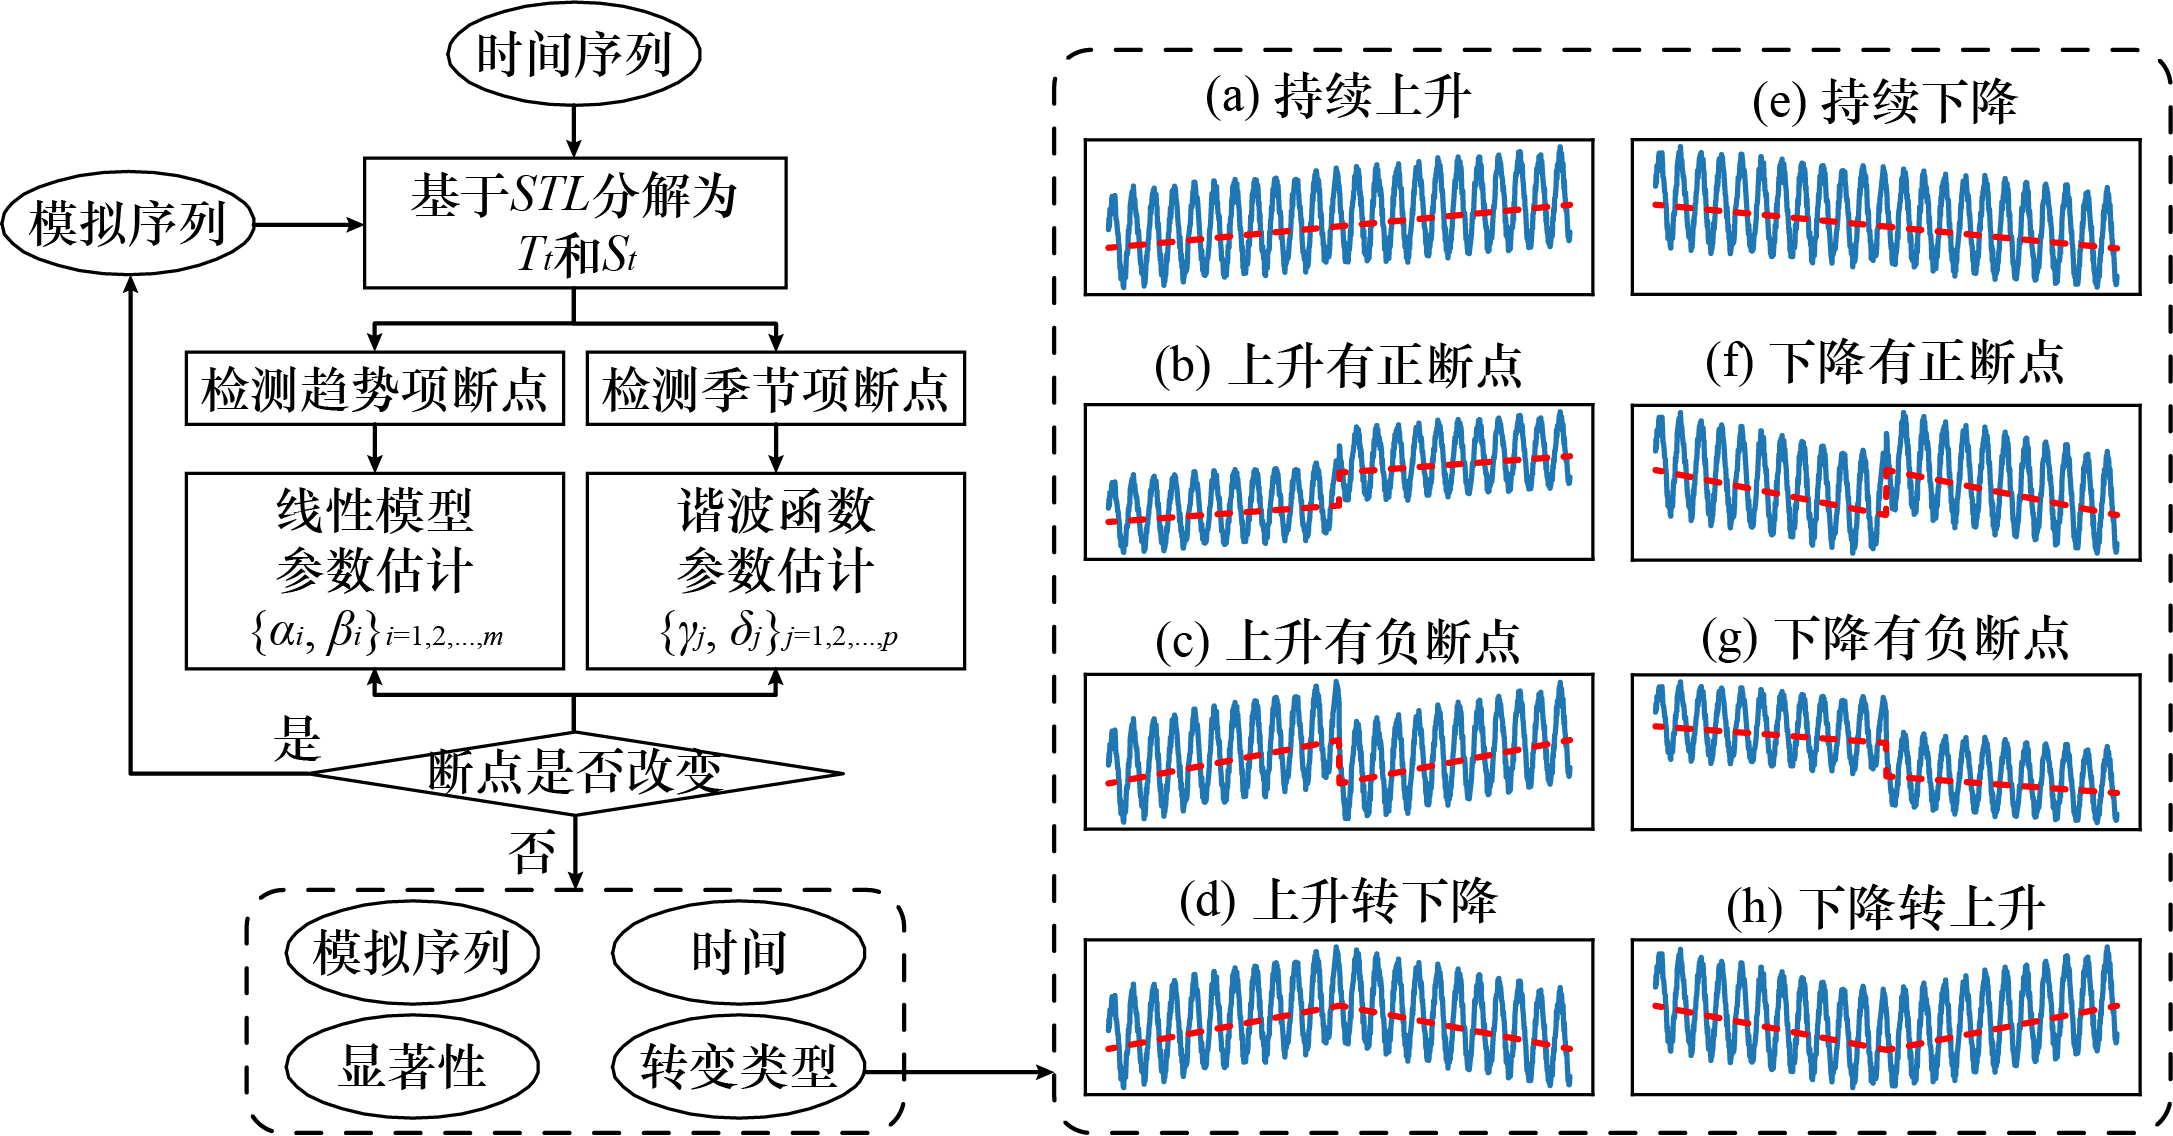
\includegraphics[width=0.9\textwidth]{figures/chap3/0_BFAST_Intro.jpg}
	\bicaption{BFAST算法流程图}{Flowchart of BFAST breakpoint detection algorithm}\label{fig:BFAST_intro}
\end{figure}

本研究使用由R语言开发的“bfast”程序包,逐站点对水文气候序列进行断点检测。程序包中,“bfast”和“bfast01”函数分别对应算法的泛化模式和变化检测模式。其中泛化模式能够指定断点数量,并基于上面介绍的分解拟合算法对原始时间序列进行模拟,变化检测模式是检测完整时间序列中是否存在一个最显著的断点,并提取断点的起始时间、变化类型、显著性等详细信息\cite{JiangPing19822015NianZhongGuoZhiBeiFuGaiBianHuaJiQiDuiQiHouBianHuaDeMinGanXingFenXi2022}。根据断点前后序列趋势变化的方向及显著性差异,“bfast01”函数将趋势变化分为8种类型,分别是:持续上升、持续下降、持续上升并有正向断点、持续上升并有负向断点、持续下降并有正向断点、持续下降并有负向断点、上升转下降、下降转上升,以提供对时间序列变化断点更详细的了解。\par

\subsection{基于数据驱动的数据缺失值插补方法}

由于BFAST断点检测算法对时间序列中缺失值敏感,为了保证算法的准确性与可执行性,需要对原始径流序列中的缺失值与无效值进行插补。由于本研究的目的是对实测径流进行分析,因此插补方法需要尽可能保留原始数据的特征,同时尽量减少插补过程中引入的不确定性。在本研究中,采用了基于数据驱动的插补方法,即基于径流序列的历史数据和其他气象要素的数据,通过数据间的相关性来插补缺失值。基于数据驱动的插补方法的基本思想是通过已有数据的特征来推断缺失数据的值,根据非缺失值时间段内的气候数据与径流观测建立联系,训练并评估机器学习模型,利用数据缺失时段的气候数据驱动训练好的模型,对缺失时段的径流进行插补。缺失径流数据插补的基本框架如图\ref{fig:Interp_Framework}所示。\par

\begin{figure}[H]
	\centering
	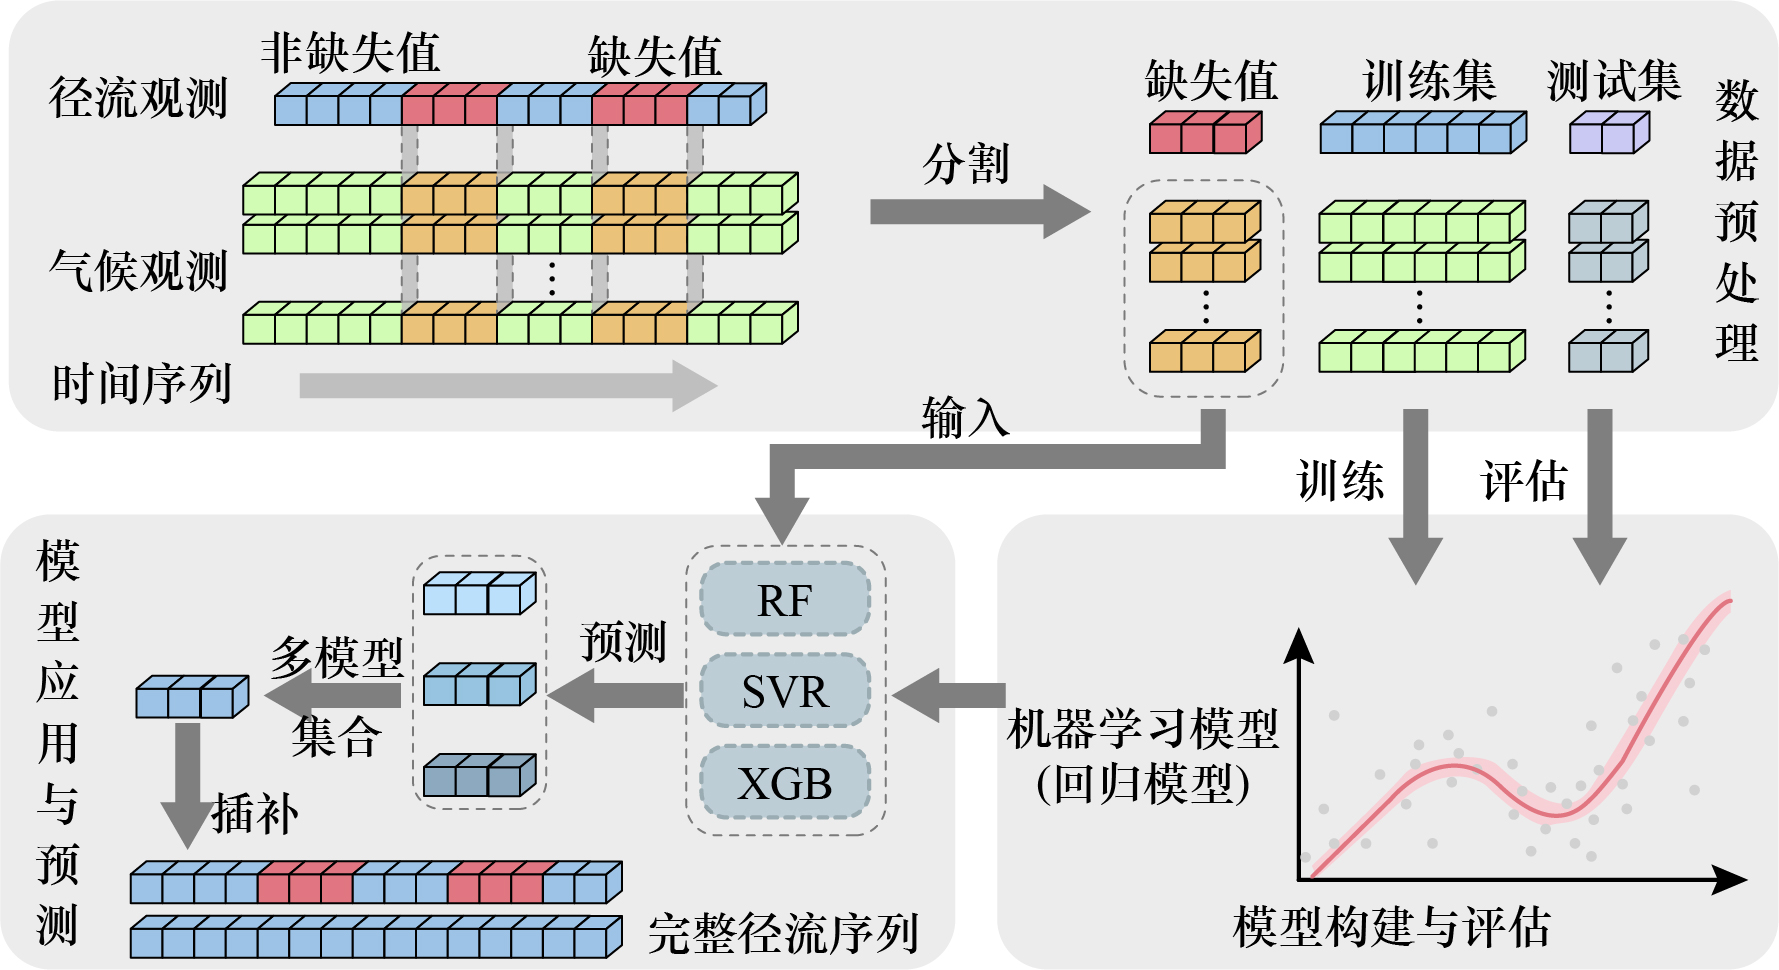
\includegraphics[width=0.85\textwidth]{figures/chap3/0_Interp_Framework.jpg}
	\bicaption{径流缺失数据插补流程图}{Interpolation flowchart of missing runoff data}
	\label{fig:Interp_Framework}
\end{figure}

本研究采用了三种常用的回归类型机器学习算法构建流域气候条件与实测径流之间的关系,分别是支持向量机回归(Support Vector Machine Regression,SVR)、随机森林(Random Forest,RF)和极端梯度提升(eXtreme Gradient Boosting,XGBoost)。这三种算法在机器学习领域中被广泛应用于回归问题,具有较好的拟合能力和泛化能力。在本研究中,对于每个流域,将径流数据作为目标变量,其他气象要素(降水、潜在蒸散发、最高气温、最低气温和平均气温)的数据作为特征变量,构建回归模型。考虑到气候条件对径流的滞后影响,每种气候变量的滞后阶数设置在0-3之间,因此有5(气象要素)×4(滞后时段)共20种特征变量。在模型训练阶段,采用了5折交叉验证的方法,以减少模型过拟合的风险。采用预测结果与实测结果的纳什效率系数(Nash-Sutcliffe Efficiency Coefficient,NSE)、相对误差(Relative Error,RE)和相关系数(Correlation Coefficient,CC),均方根误差(Root Mean Square Error,RMSE)作为评价指标,以评估模型的模拟结果与泛化能力。

\begin{equation}
    \label{equ:NSE}
	NSE=1-\frac{\sum_{t=1}^{n}\left(Q o_{i}-Q s_{i}\right)^{2}}{\sum_{t=1}^{n}\left(Q o_{i}-\overline{Q o}\right)^{2}}
\end{equation}

\begin{equation}
    \label{equ:RE}
	RE=\frac{\overline{Q_s}-\overline{Q_o}}{\overline{Q_o}}
\end{equation}

\begin{equation}
    \label{equ:CC}
	CC=\frac{\sum_{t=1}^{n}((Q_{o_i}-\overline{Q_o})(Q_{s_i}-\overline{Q_s}))}{\sqrt{\sum_{t=1}^{n}(Q_{o_i}-\overline{Q_o})^2\sum_{t=1}^{n}(Q_{s_i}-\overline{Q_s})^2}} 
\end{equation}

\begin{equation}
    \label{equ:RMSE}
	RMSE=\sqrt{ \sum_{t=1}^{n}\frac{(Q_{s_i}-Q_{o_i})^2}{n} }  
\end{equation}

式中$Q_o$和$Q_s$分别代表了观测值和模拟值,$\overline{Q_o}$和$\overline{Q_s}$分别代表了观测值和模拟值的平均值,$n$为样本数量。\par
在模型应用阶段,利用数据缺失时段的气候数据驱动训练好的模型,预测缺失时段的径流数据。为了减少模型预测结果的不确定性,对于每个流域,采用三种机器学习算法分别进行插补,最终插补结果取三种算法的平均值作为最终插补结果。\par

% \subsection{径流变化归因分析方法}

% \subsubsection{多年尺度径流变化归因分析方法}

% \subsubsection{径流年内变异性归因分析方法}

% \section{全球历史气候要素时空演变格局}

% \subsection{全球气候要素时空变化特征}

% \begin{figure}[H]
% 	\centering
% 	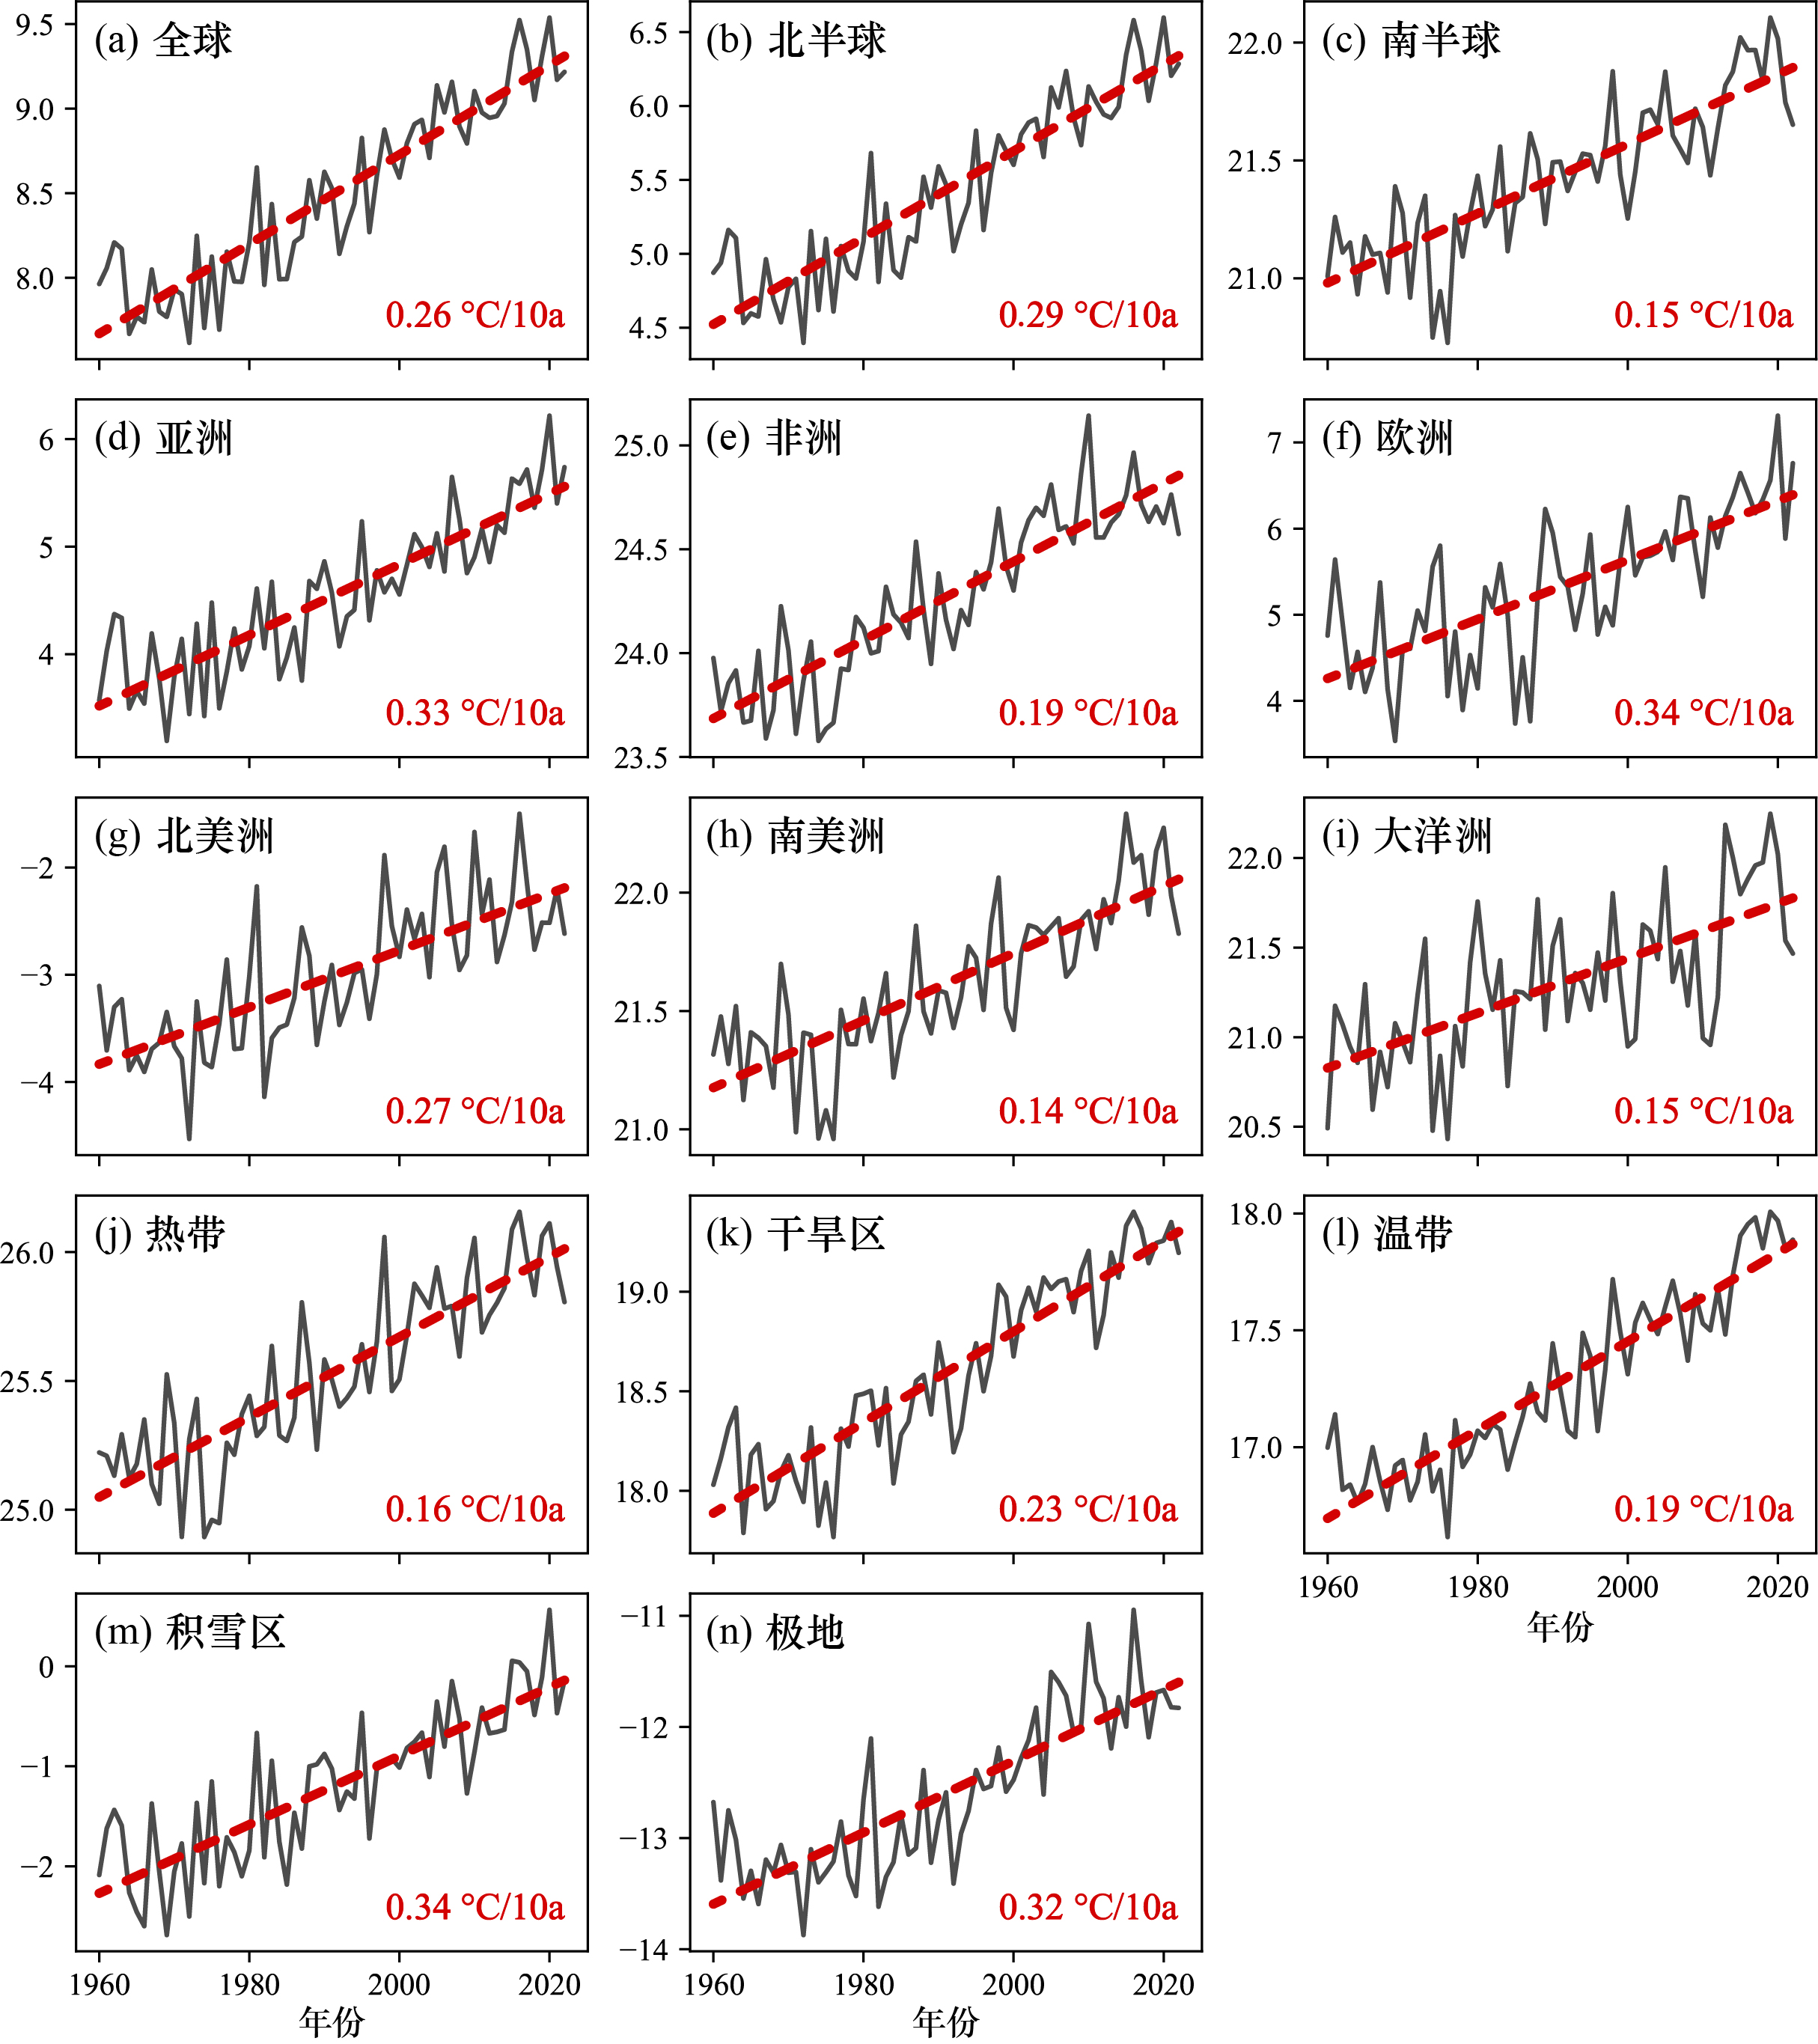
\includegraphics[width=0.85\textwidth]{figures/chap3/1_TEM_Series.jpg}
% 	\bicaption{全球及区域气温序列及变化趋势}{Temperature series and linear trend in global and regional scale}
% 	\label{fig:TEM_Series}
% \end{figure}

% \begin{figure}[H]
% 	\centering
% 	\includegraphics[width=0.85\textwidth]{figures/chap3/1_TT.jpg}
% 	\bicaption{全球年、季尺度气温变化空间格局}{Spatial pattern of annual and seasonal temperature trend}
% 	\label{fig:TEM_Trend_Map}
% \end{figure}

% \begin{figure}[H]
% 	\centering
% 	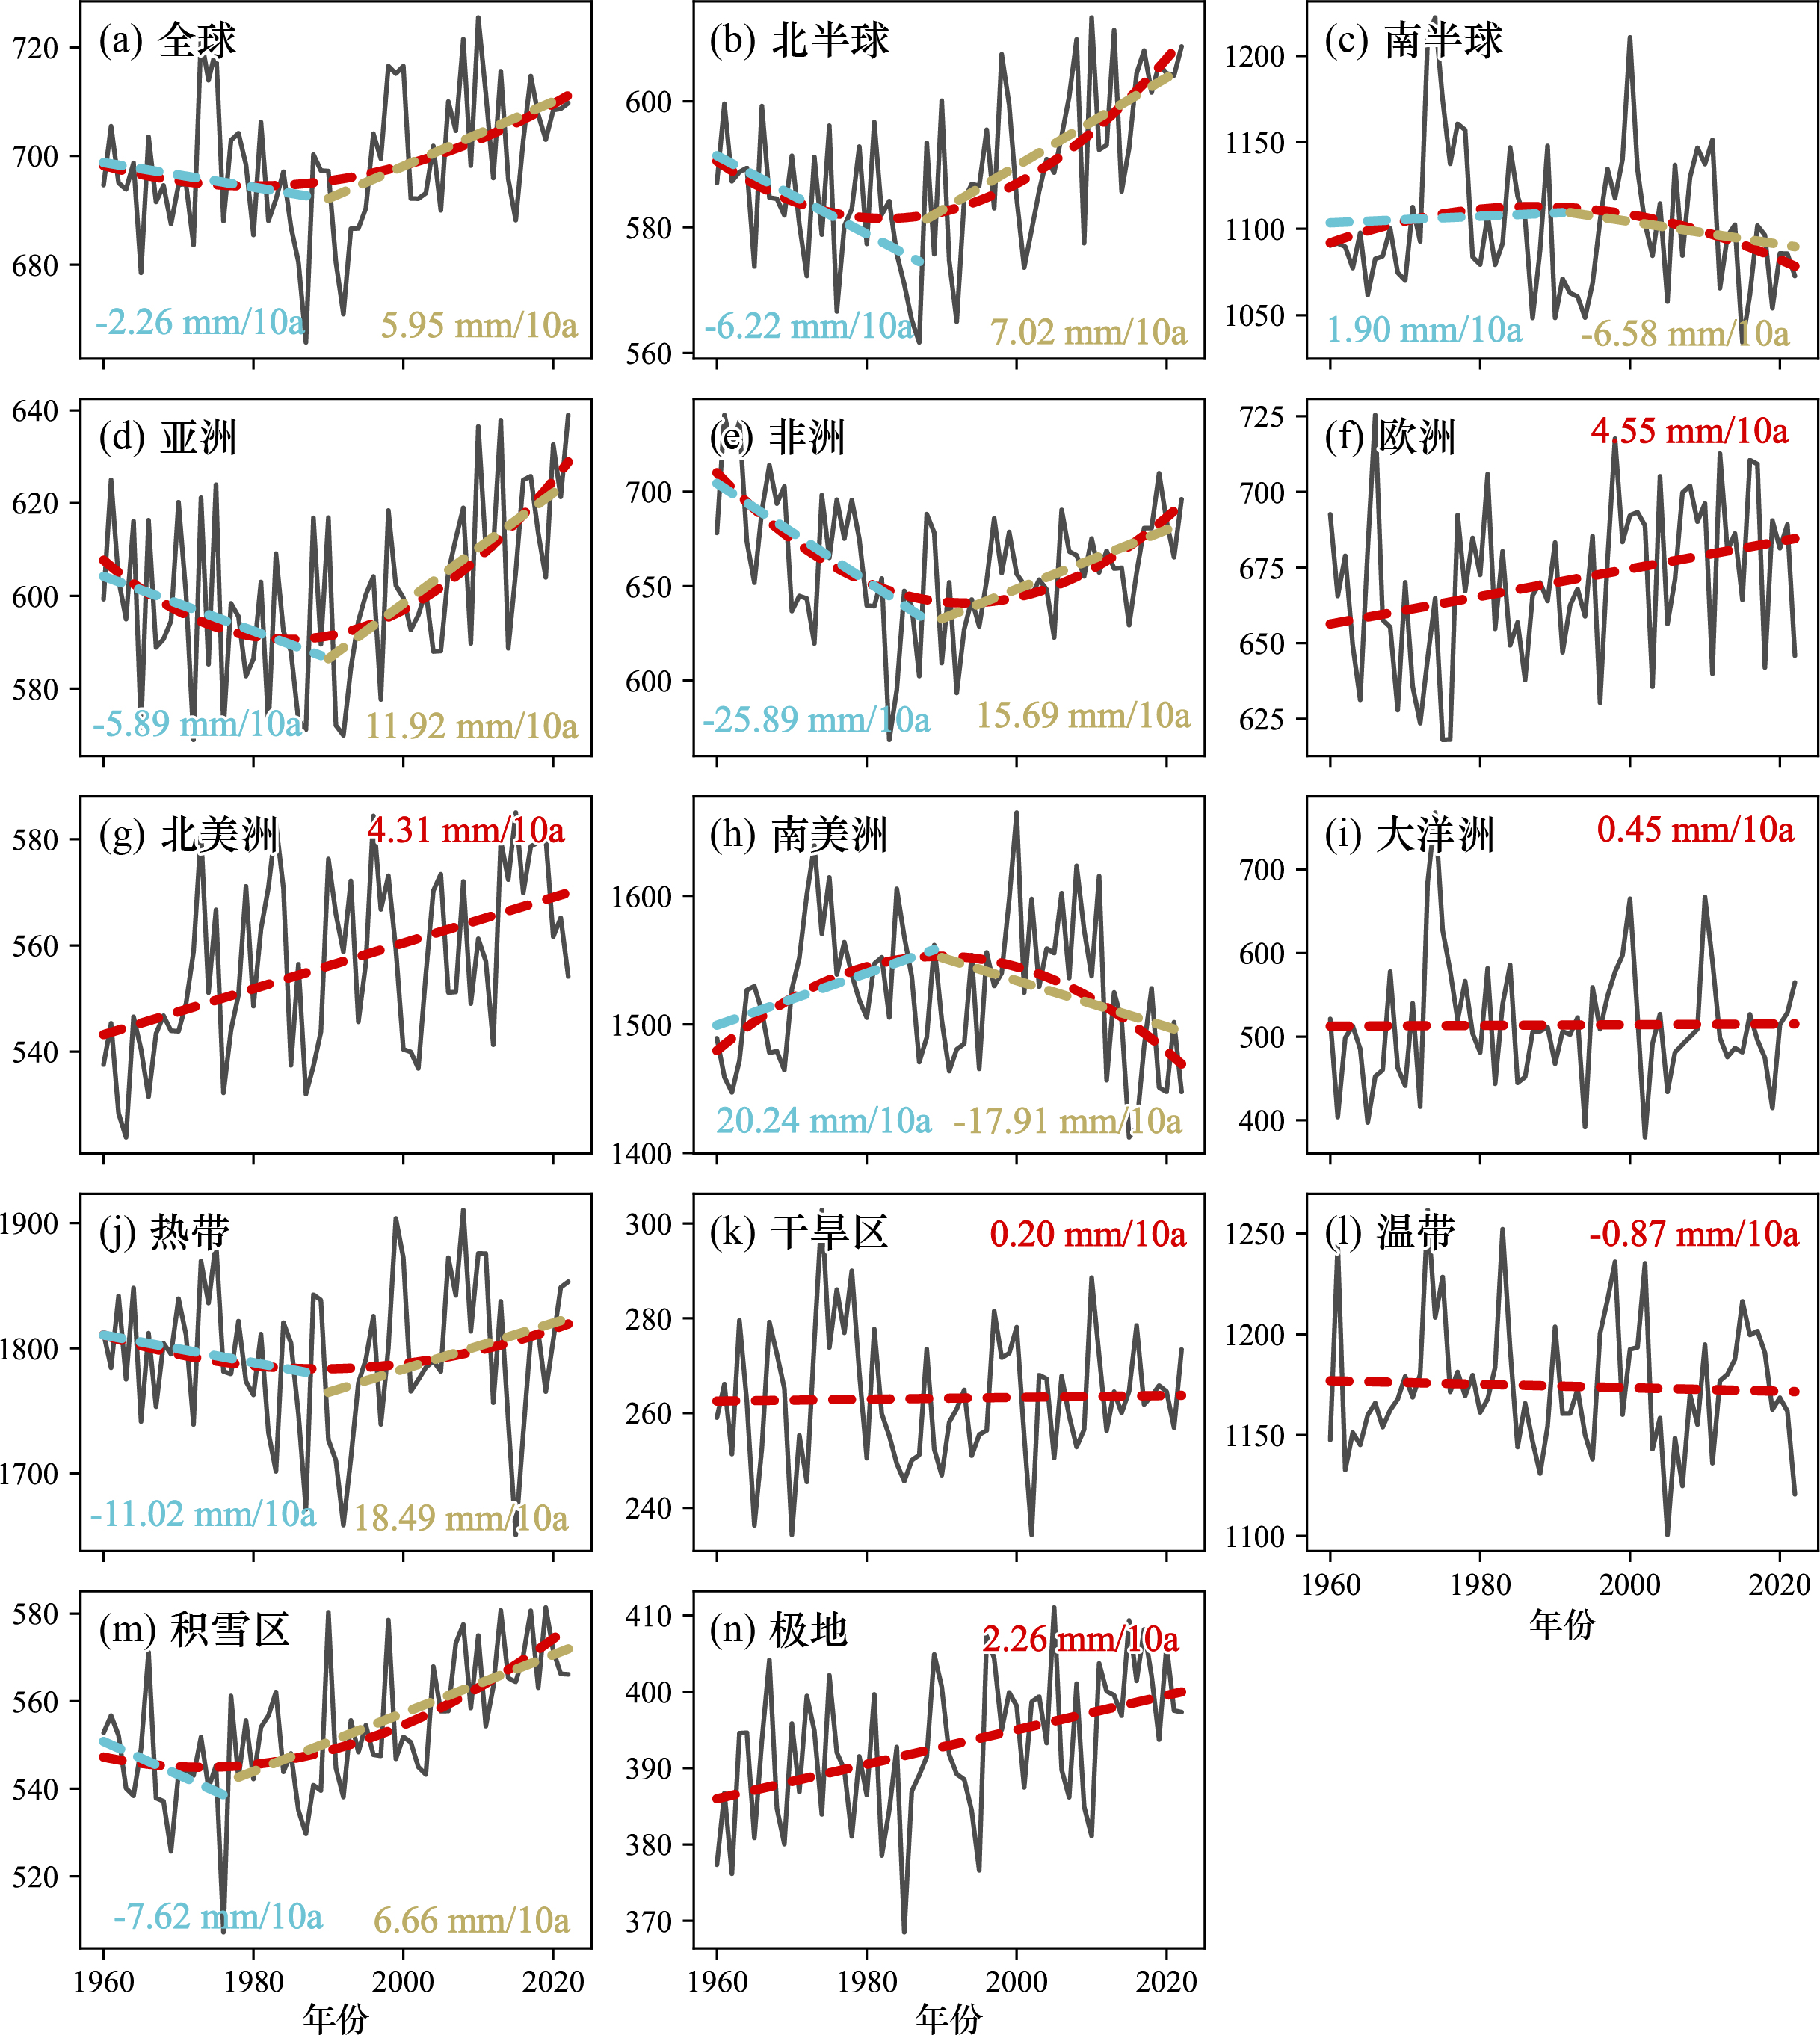
\includegraphics[width=0.85\textwidth]{figures/chap3/1_PRE_Series.jpg}
% 	\bicaption{全球及区域降水序列及变化趋势}{Precipitation series and linear trend in global and regional scale}
% 	\label{fig:PRE_Series}
% \end{figure}

% \begin{figure}[H]
% 	\centering
% 	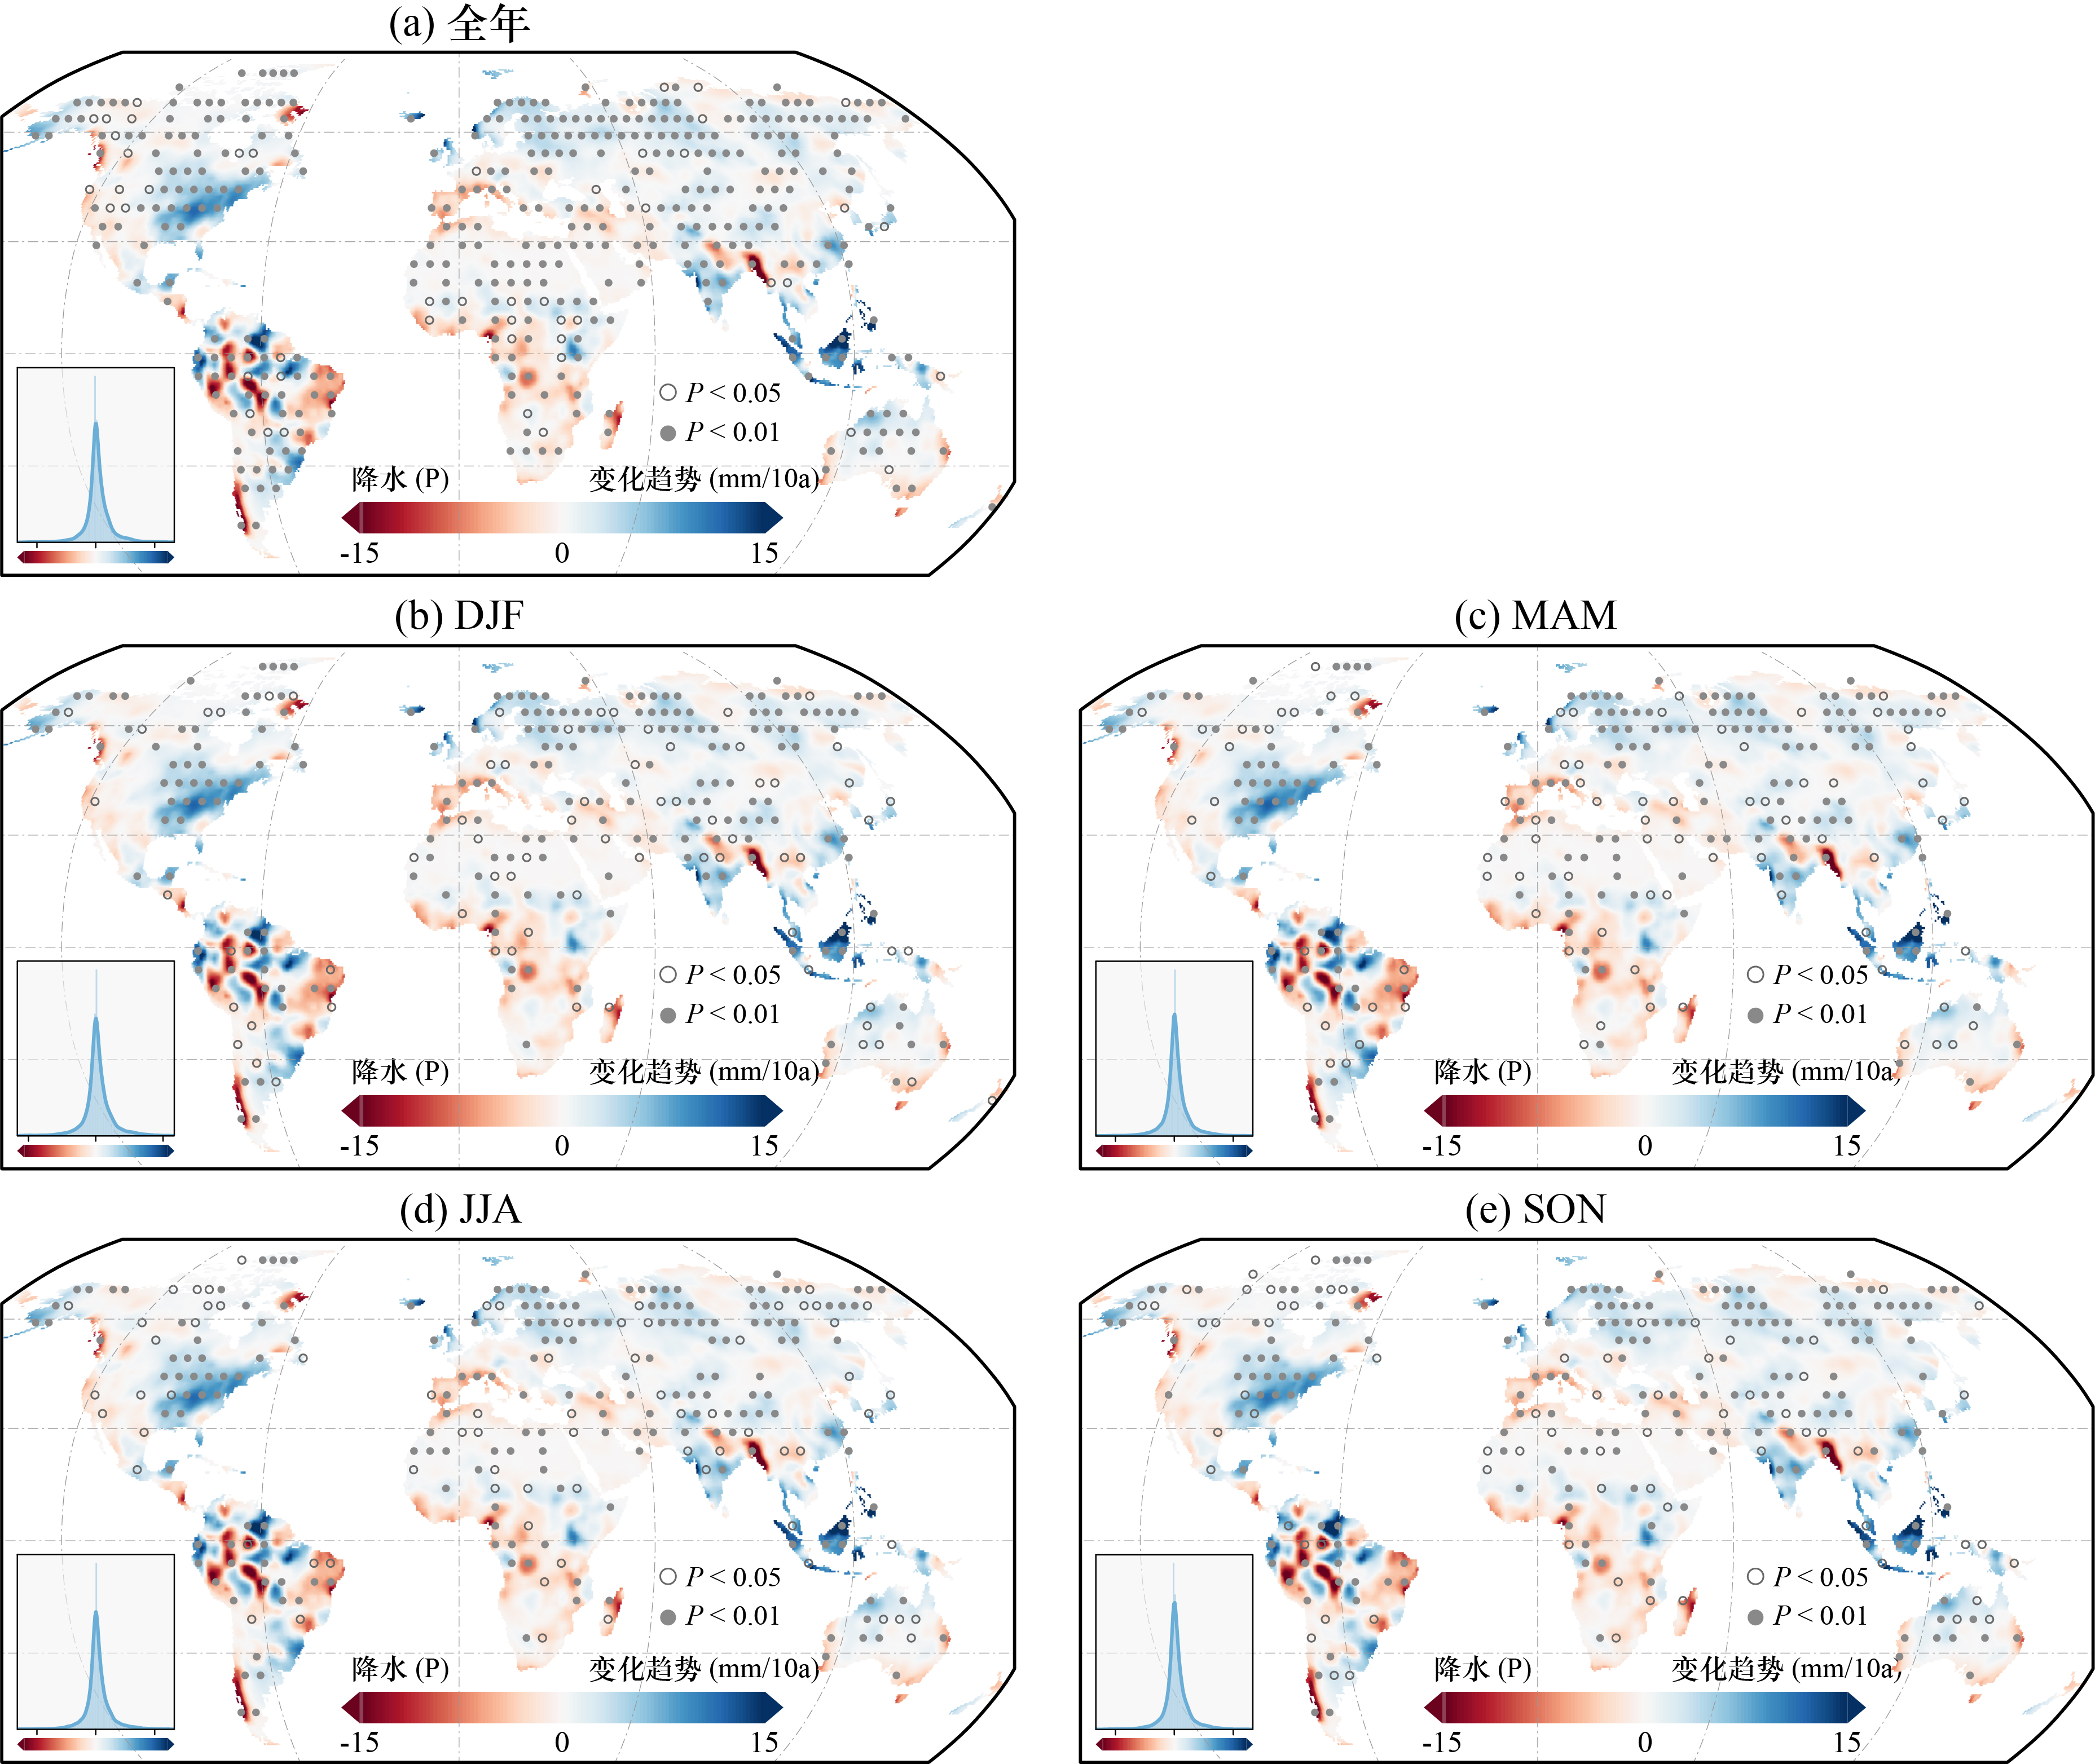
\includegraphics[width=0.85\textwidth]{figures/chap3/1_PT.jpg}
% 	\bicaption{全球年、季尺度降水变化空间格局}{Spatial pattern of annual and seasonal precipitation trend}
% 	\label{fig:PRE_Trend_Map}
% \end{figure}

% \begin{figure}[H]
% 	\centering
% 	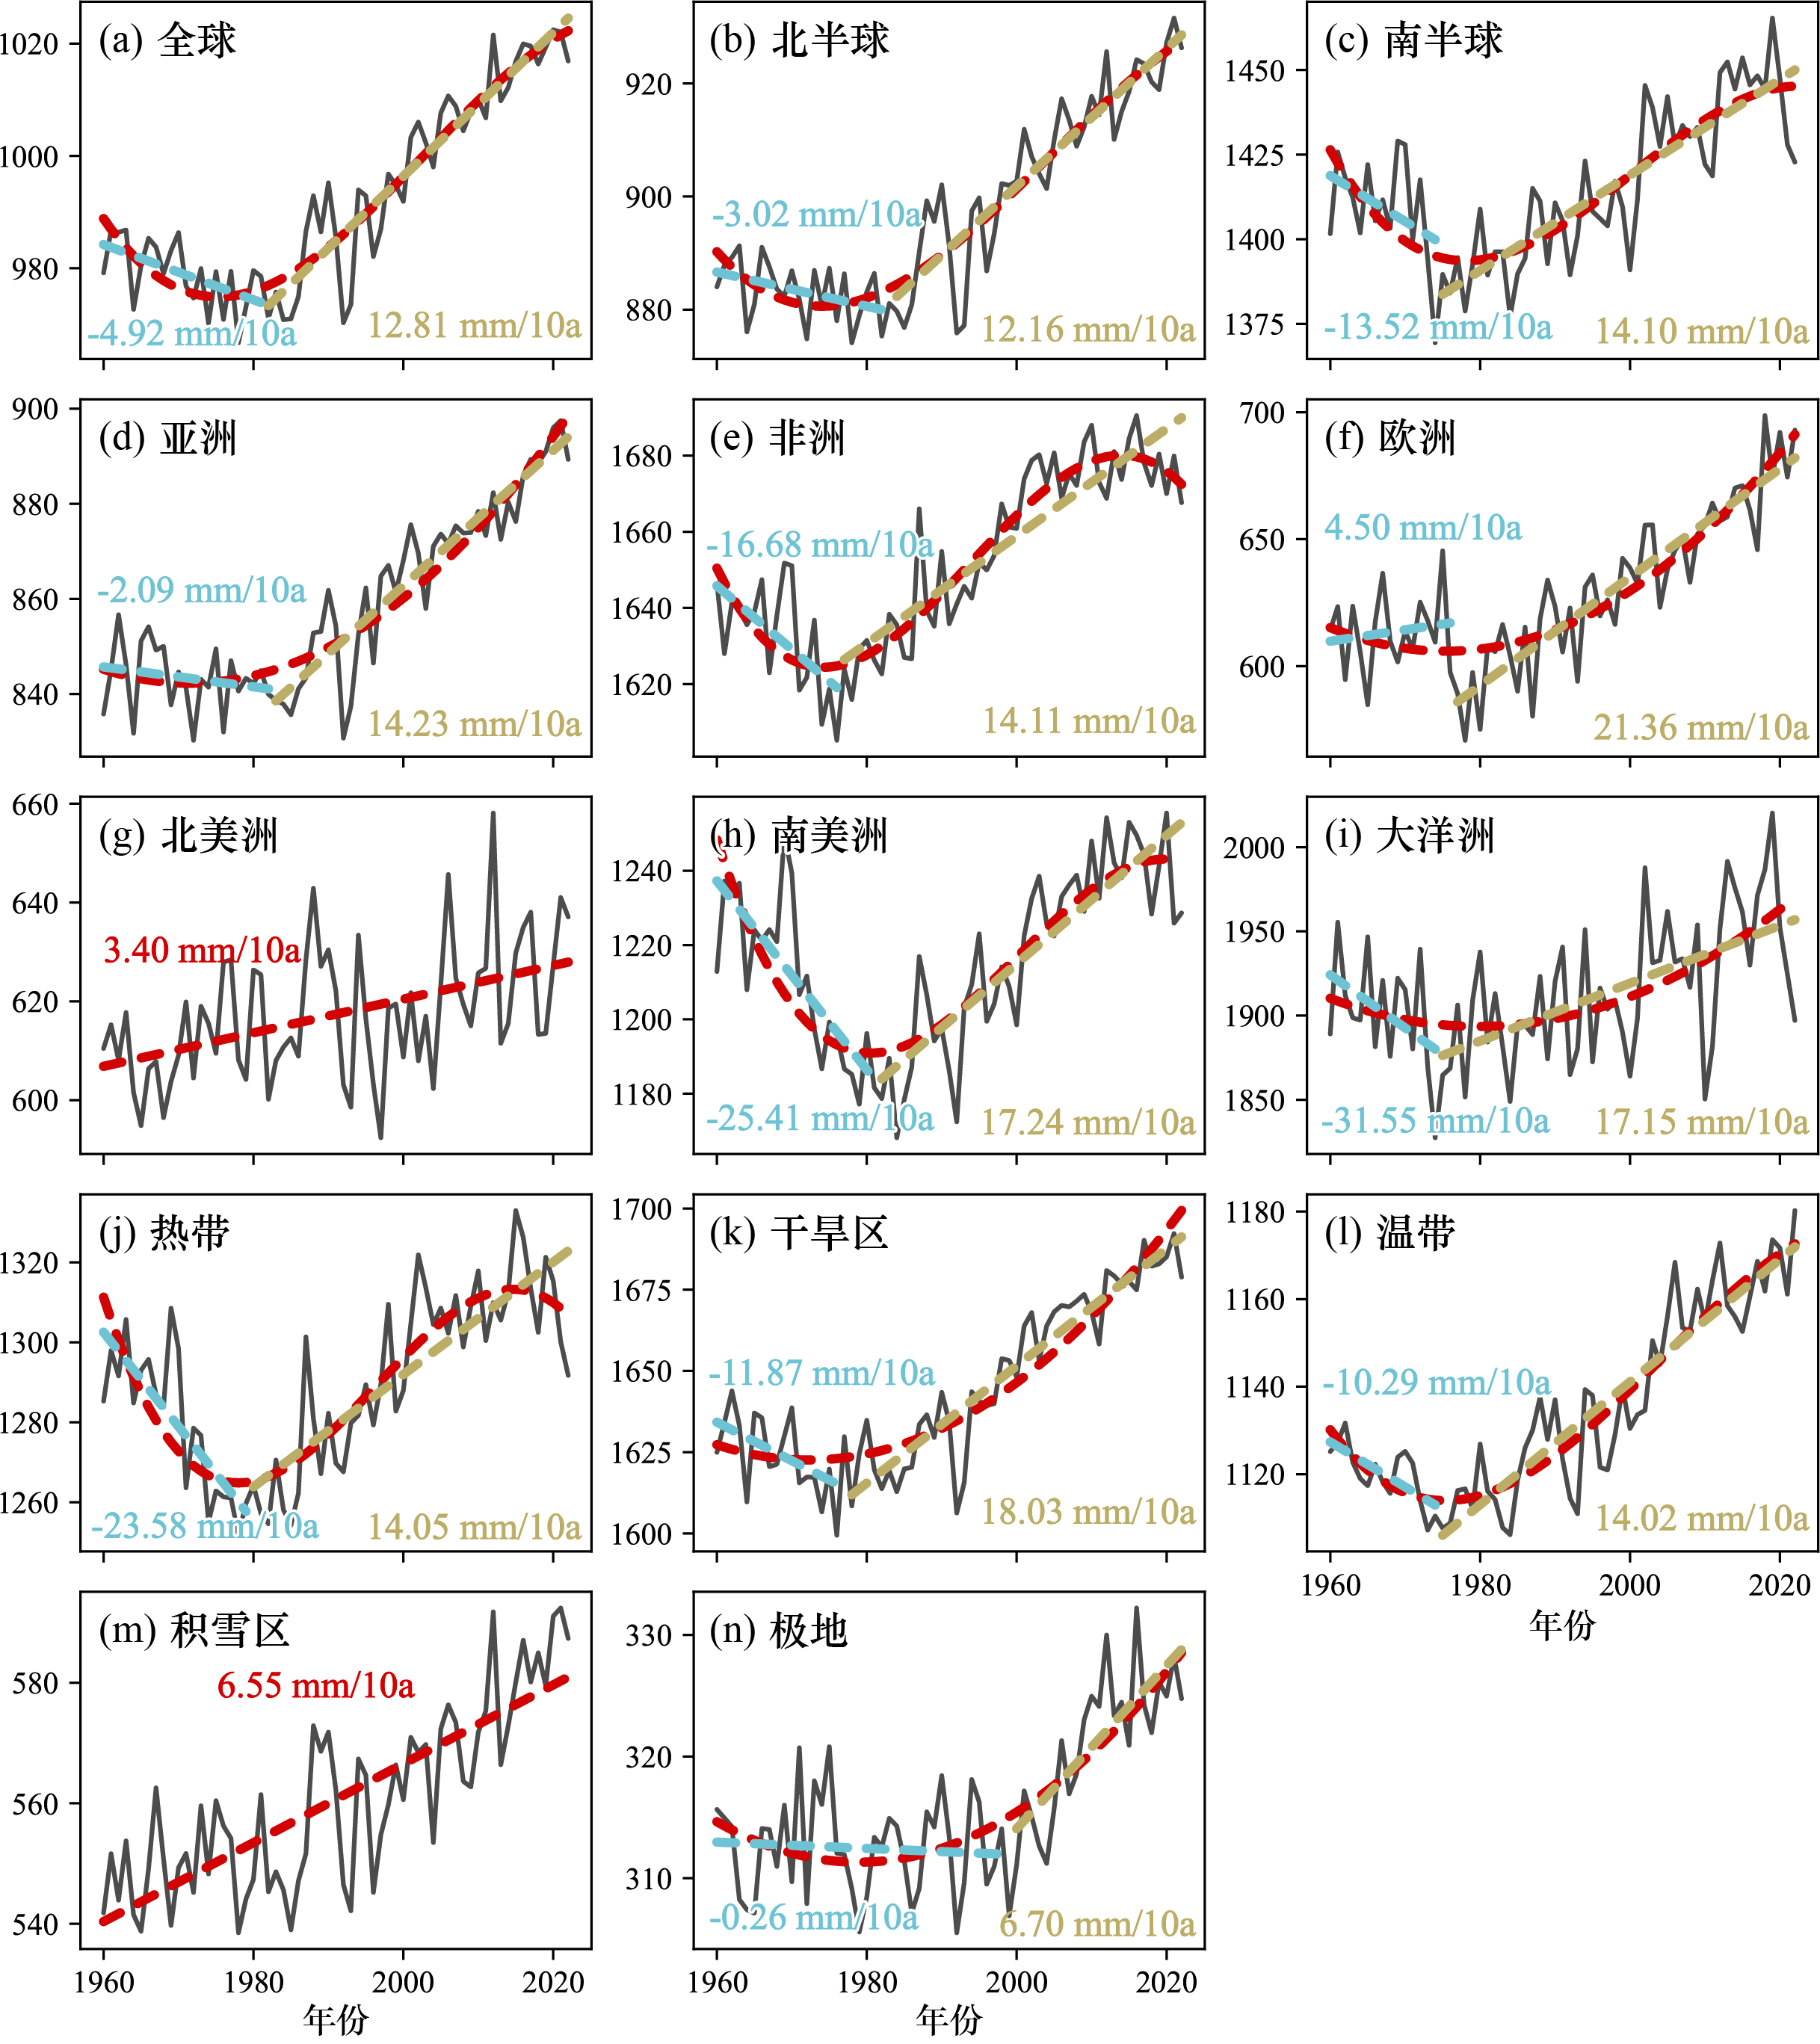
\includegraphics[width=0.85\textwidth]{figures/chap3/1_PET_Series.jpg}
% 	\bicaption{全球及区域潜在蒸散发序列及变化趋势}{Potential evapotranspiration series and linear trend in global and regional scale}
% 	\label{fig:PET_Series}
% \end{figure}

% \begin{figure}[H]
% 	\centering
% 	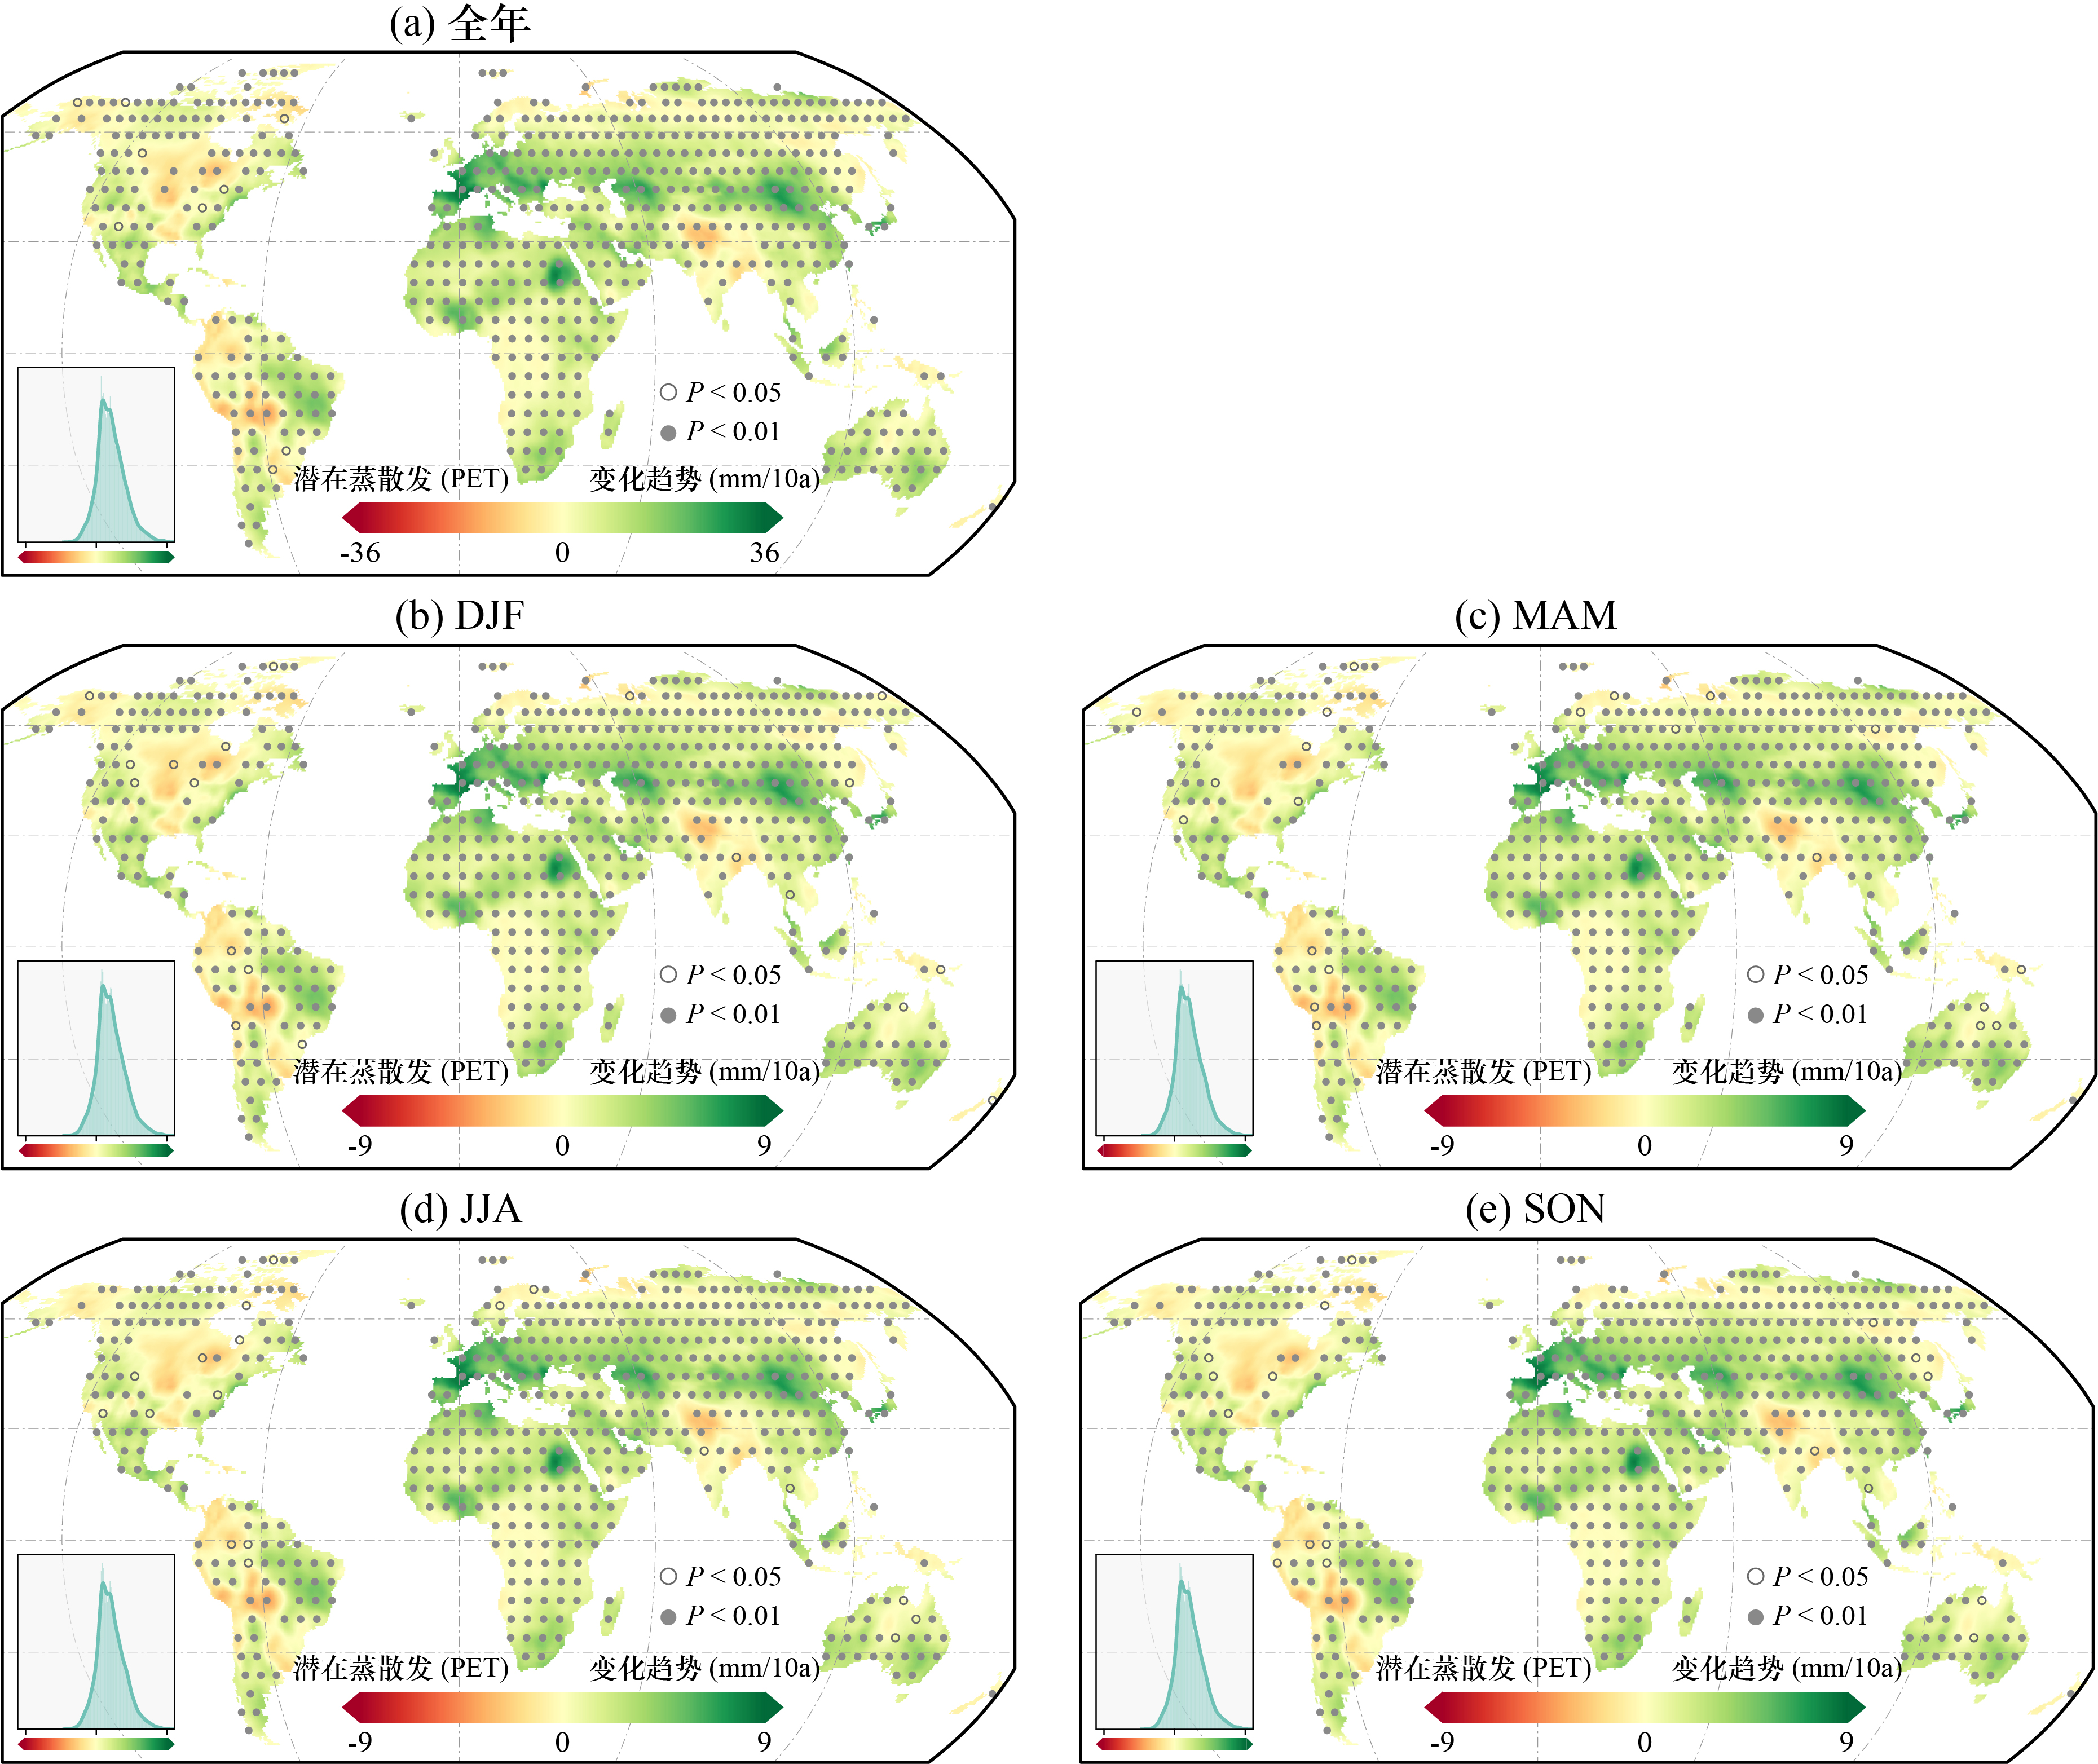
\includegraphics[width=0.85\textwidth]{figures/chap3/1_ET.jpg}
% 	\bicaption{全球年、季尺度潜在蒸散发变化空间格局}{Spatial pattern of annual and seasonal potential evapotranspiration trend}
% 	\label{fig:PET_Trend_Map}
% \end{figure}

% \begin{figure}[H]
% 	\centering
% 	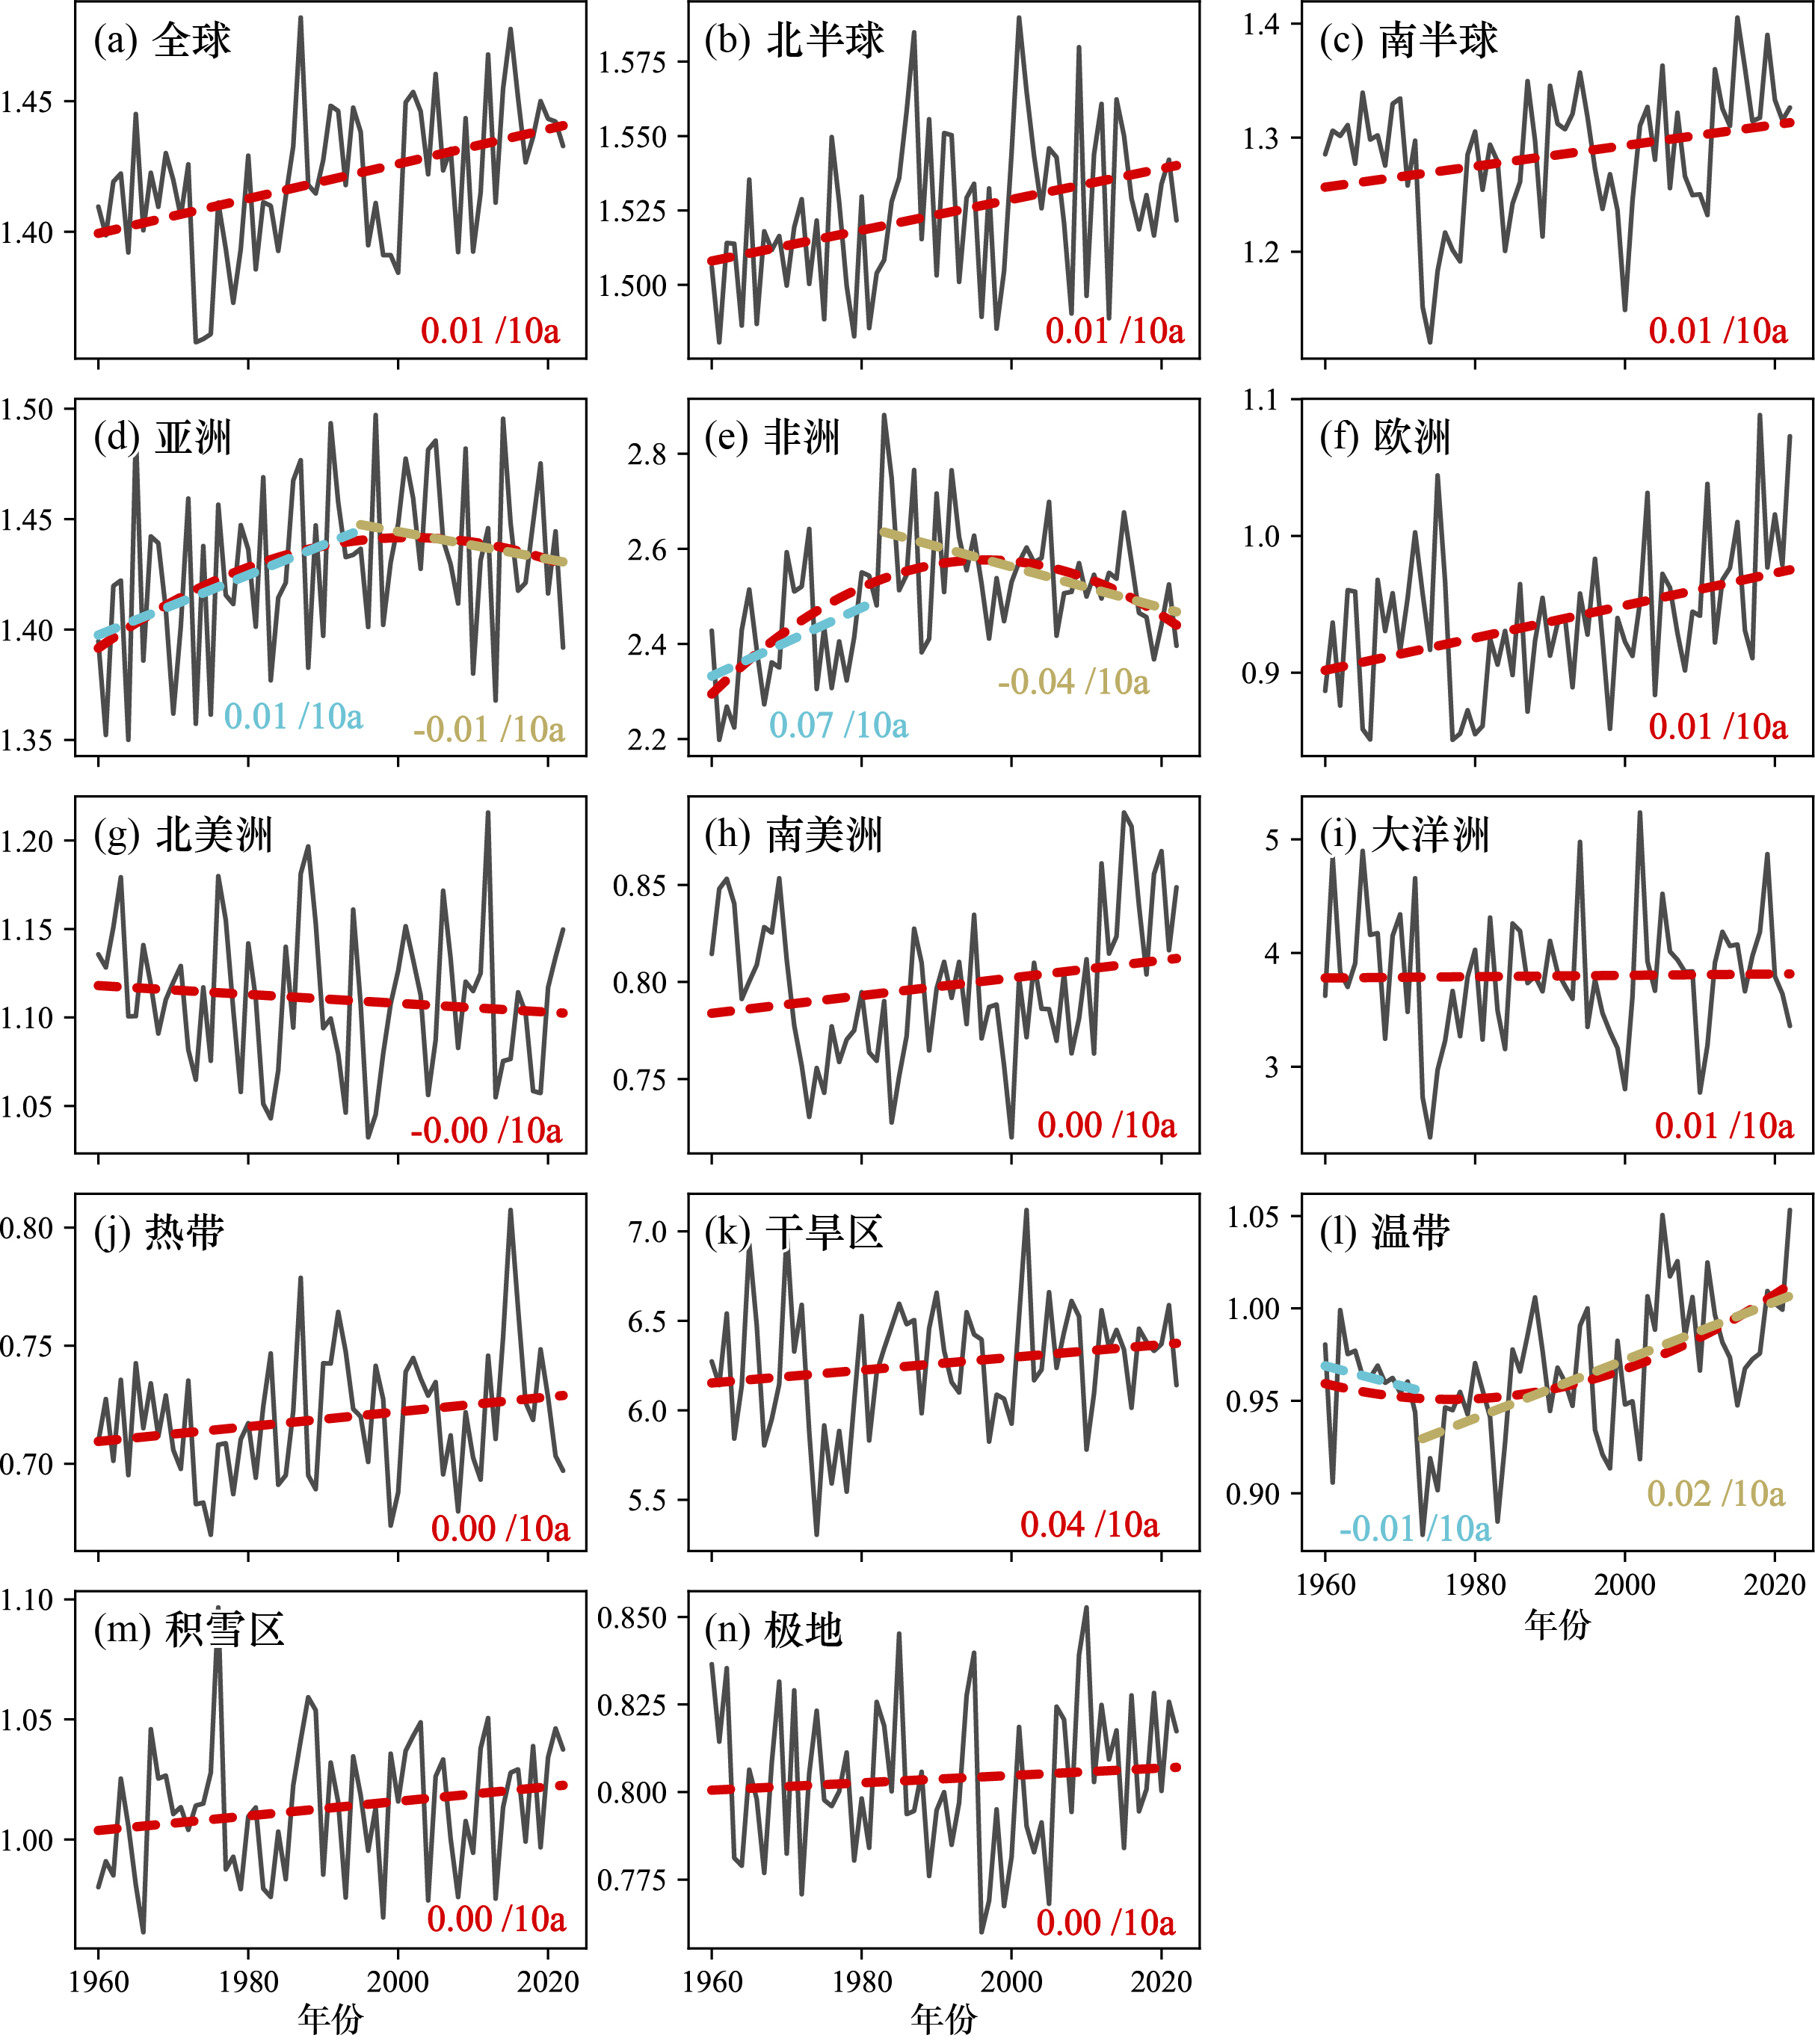
\includegraphics[width=0.85\textwidth]{figures/chap3/1_AI_Series.jpg}
% 	\bicaption{全球及区域干燥度指数序列及变化趋势}{Aridity index series and linear trend in global and regional scale}
% 	\label{fig:AI_Series}
% \end{figure}

% \begin{figure}[H]
% 	\centering
% 	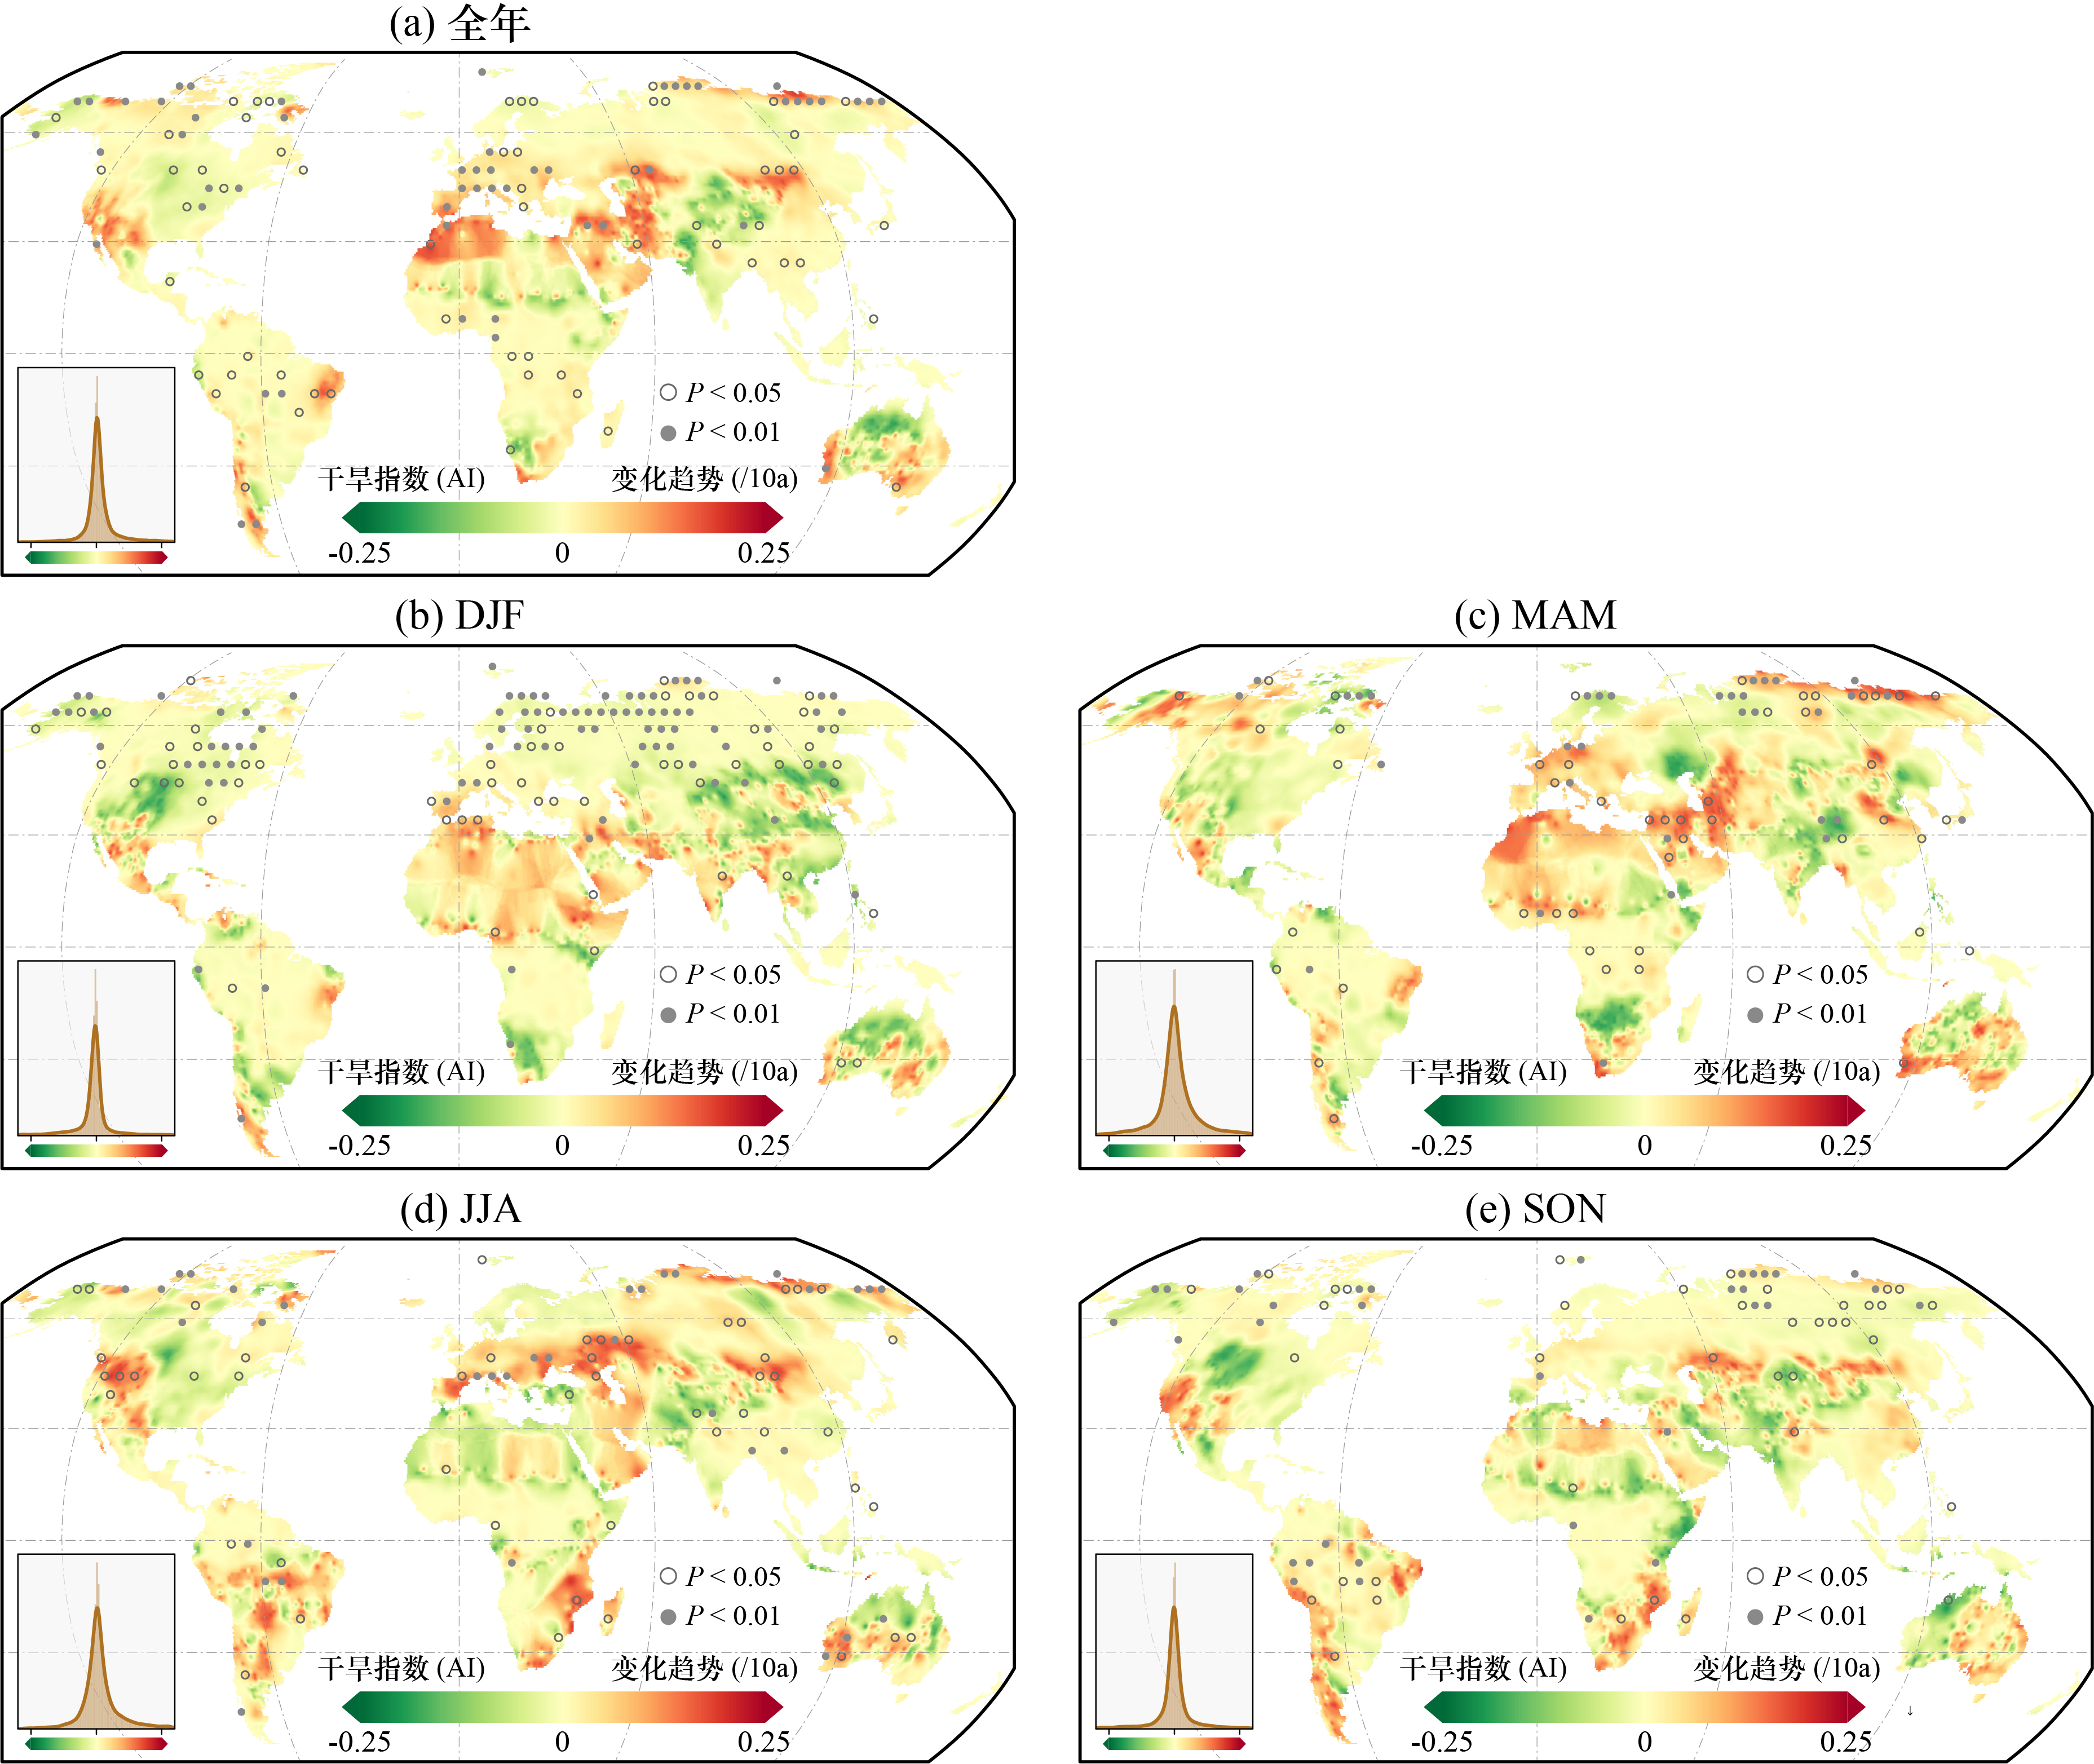
\includegraphics[width=0.85\textwidth]{figures/chap3/1_AT.jpg}
% 	\bicaption{全球年、季尺度干燥度指数变化空间格局}{Spatial pattern of annual and seasonal aridity index trend}
% 	\label{fig:AI_Trend_Map}
% \end{figure}

% \begin{figure}[H]
% 	\centering
% 	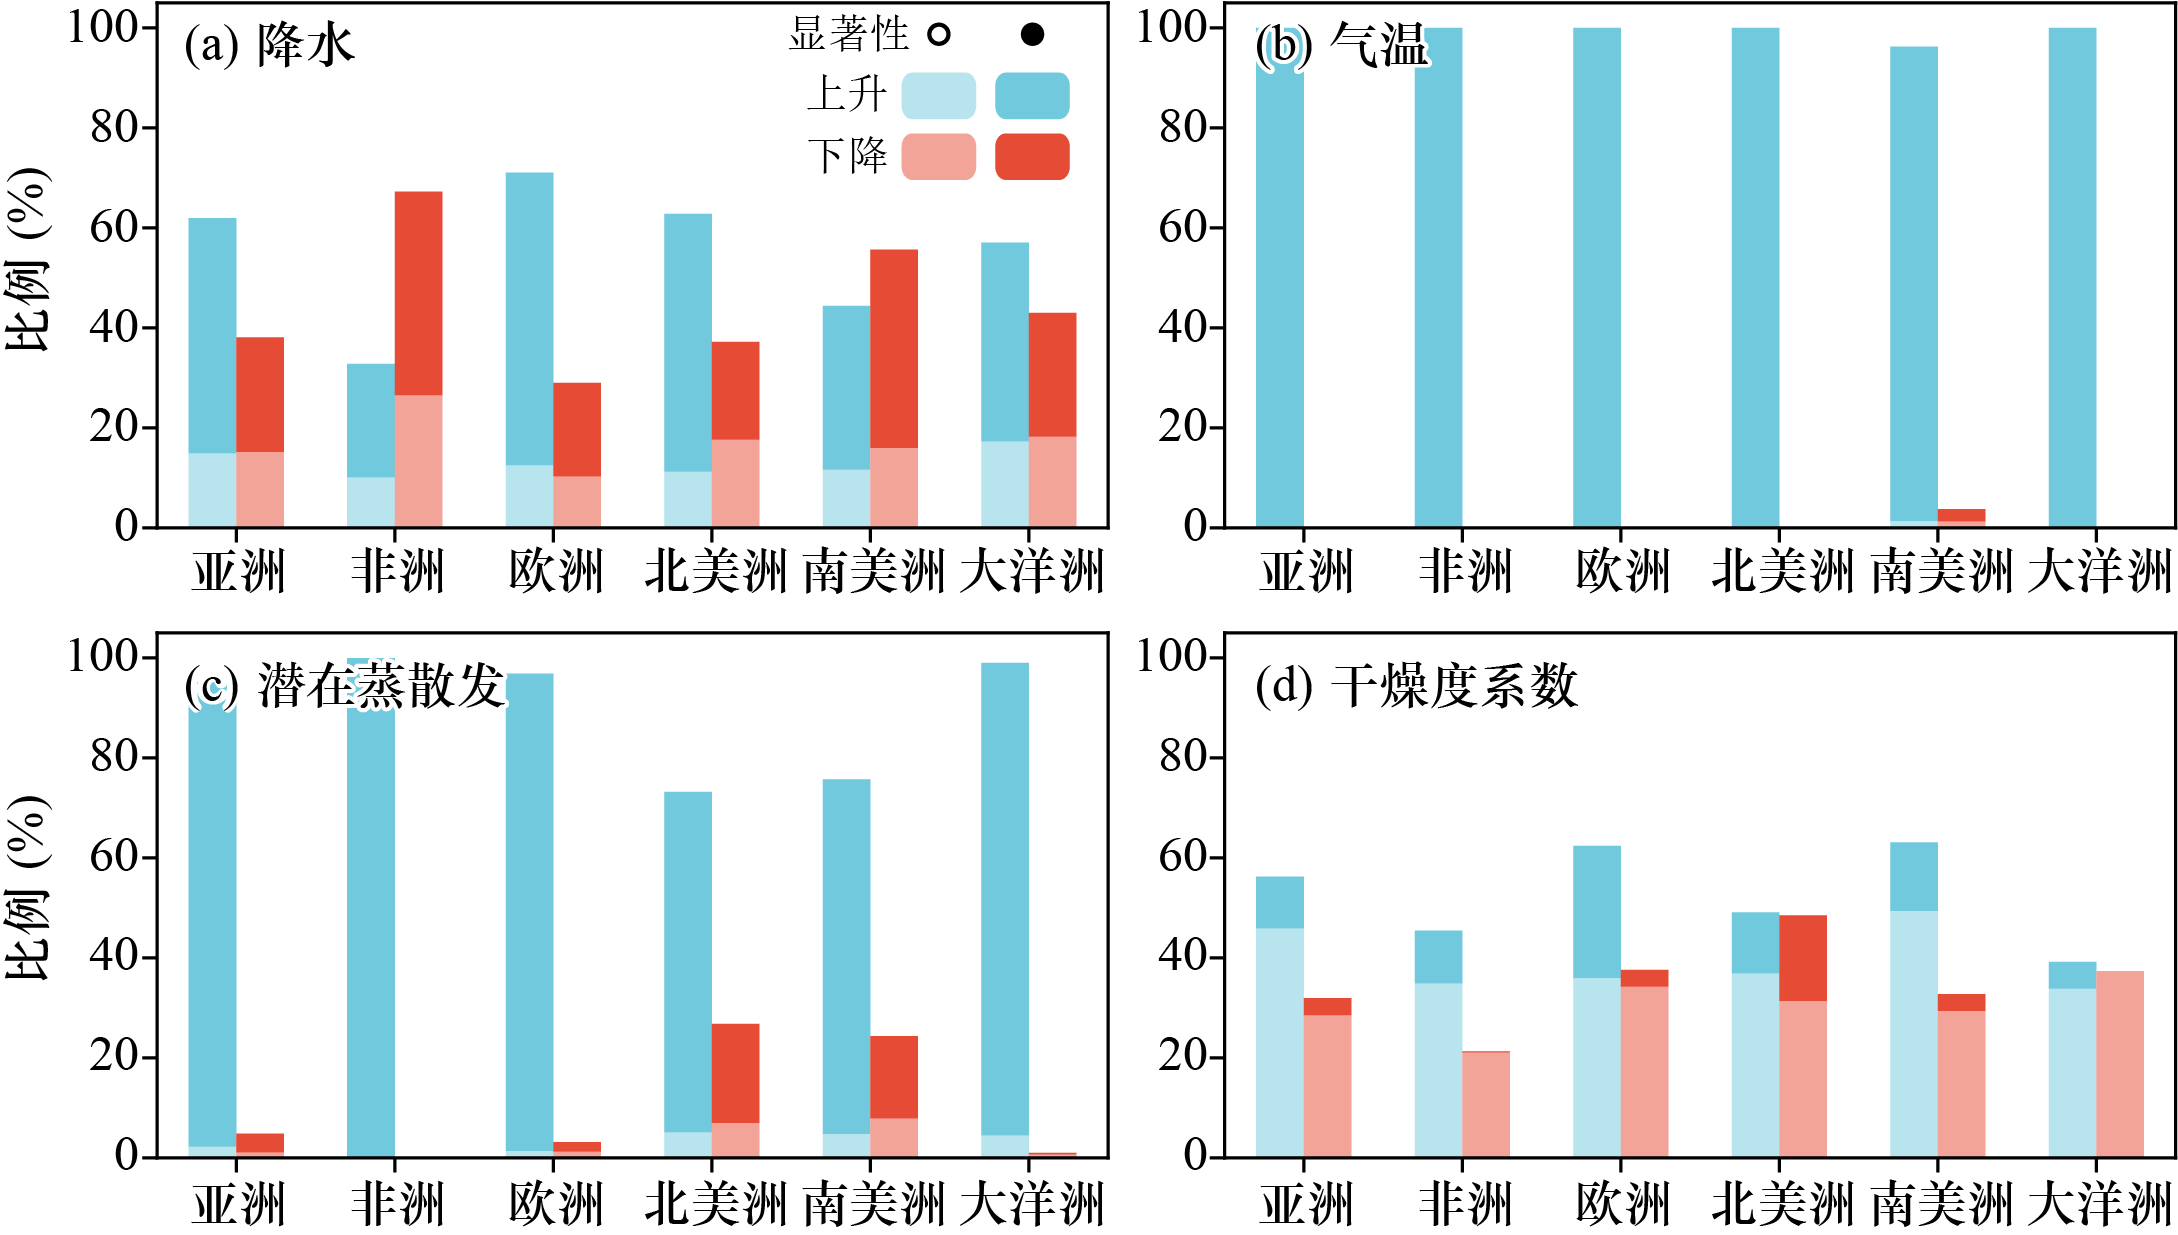
\includegraphics[width=0.85\textwidth]{figures/chap3/1_Trend_Stat_Conti.jpg}
% 	\bicaption{各大洲气候要素变化趋势统计}{Statistic of climatic contidions change for each continents}
% 	\label{fig:Trend_Stat_Conti}
% \end{figure}

% \begin{figure}[H]
% 	\centering
% 	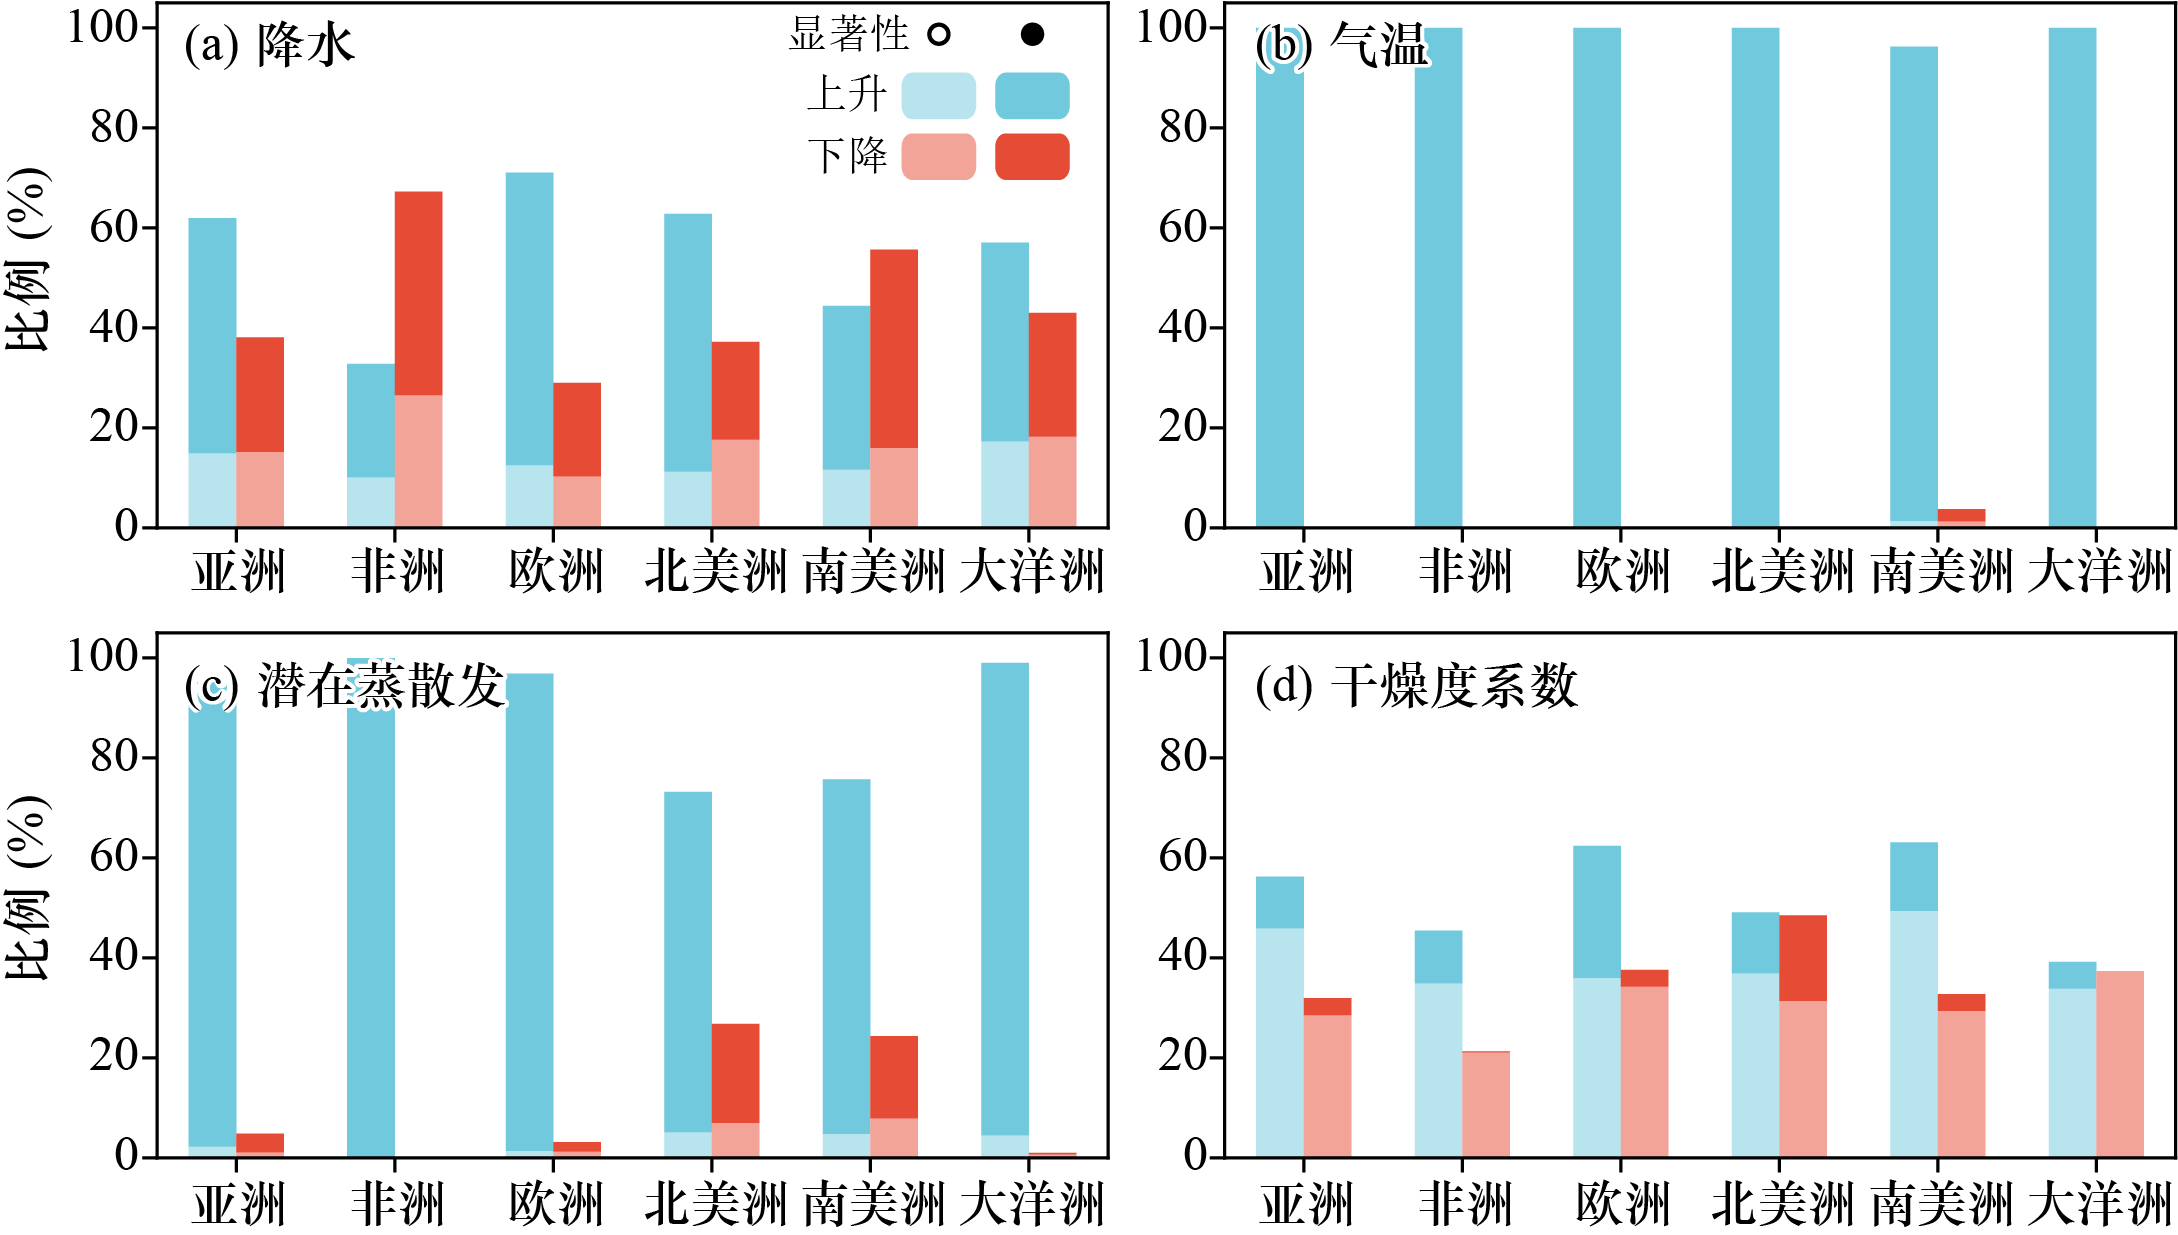
\includegraphics[width=0.85\textwidth]{figures/chap3/1_Trend_Stat_Conti.jpg}
% 	\bicaption{各气候区气候要素变化趋势统计}{Statistic of climatic contidions change for each climatic zones}
% 	\label{fig:Trend_Stat_Clim}
% \end{figure}

% \subsection{区域尺度气候要素的线性-非线性演变特征}

% \begin{figure}[H]
% 	\centering
% 	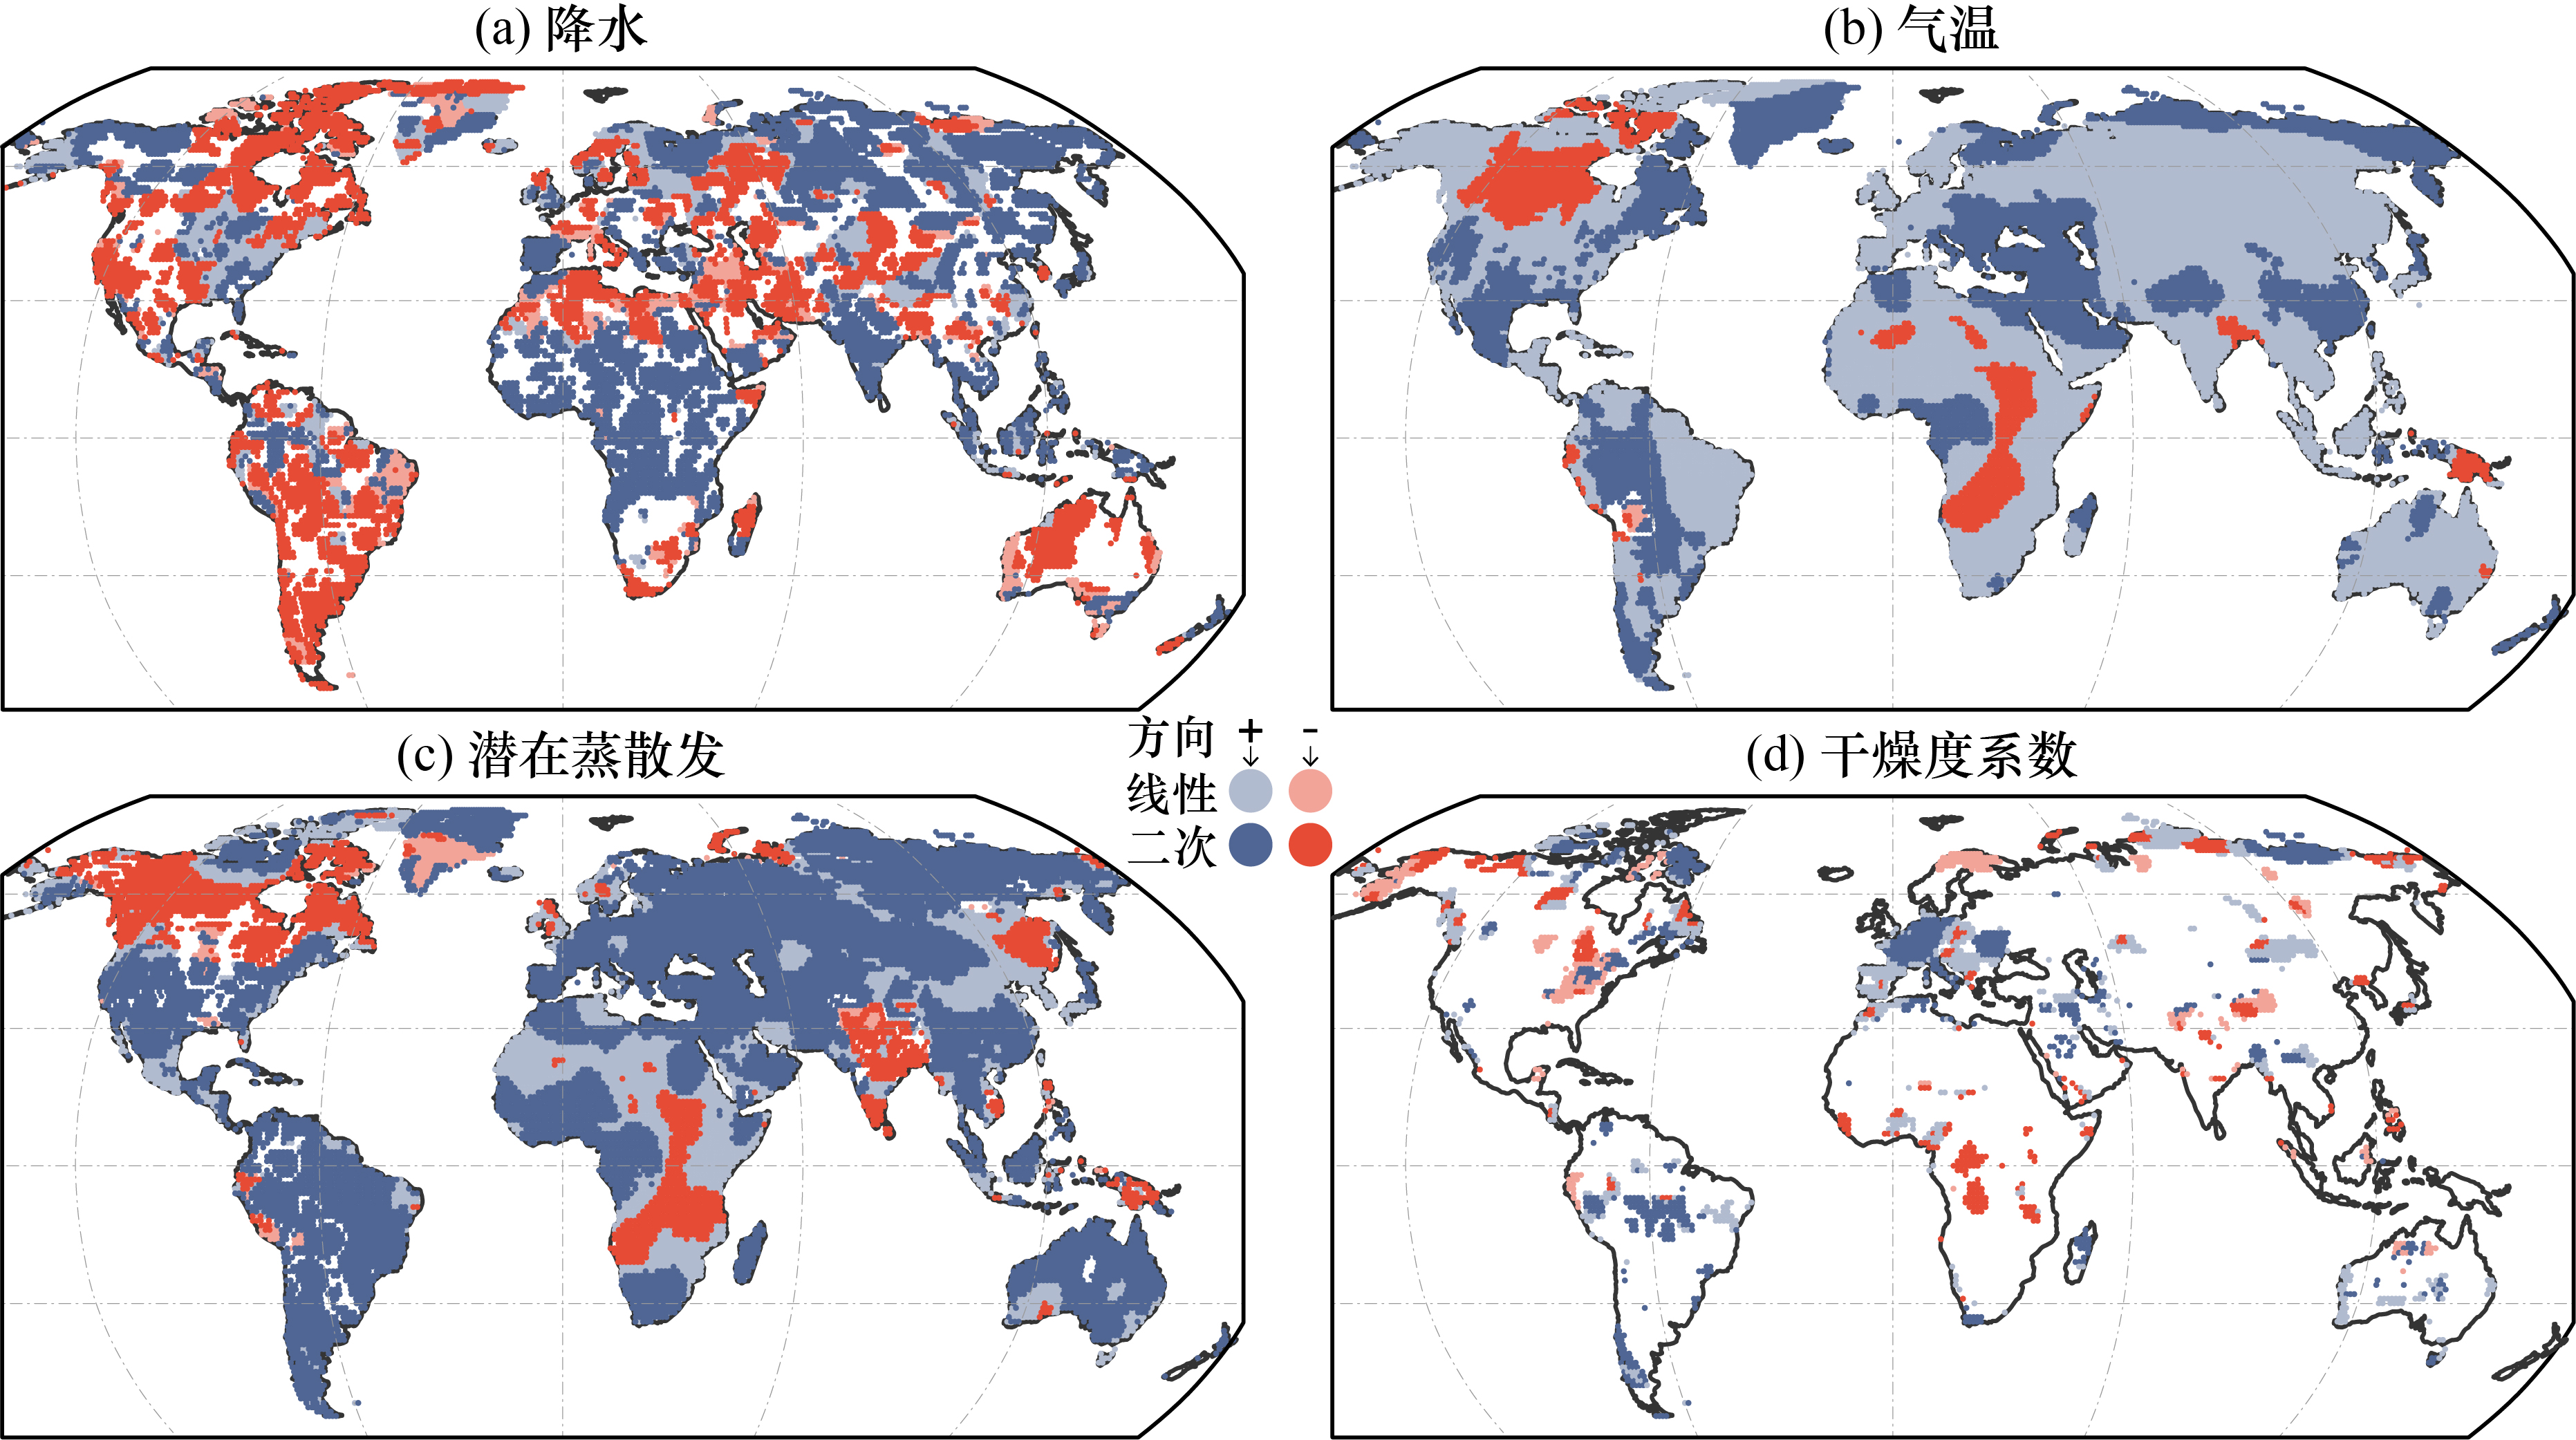
\includegraphics[width=0.85\textwidth]{figures/chap3/1_LNL_Map.jpg}
% 	\bicaption{全球气候要素线性-非线性变化空间格局}{Spatial pattern of climatic trend direction and linear-nonlinear trend type}
% 	\label{fig:LNL_Map}
% \end{figure}

% \begin{figure}[H]
% 	\centering
% 	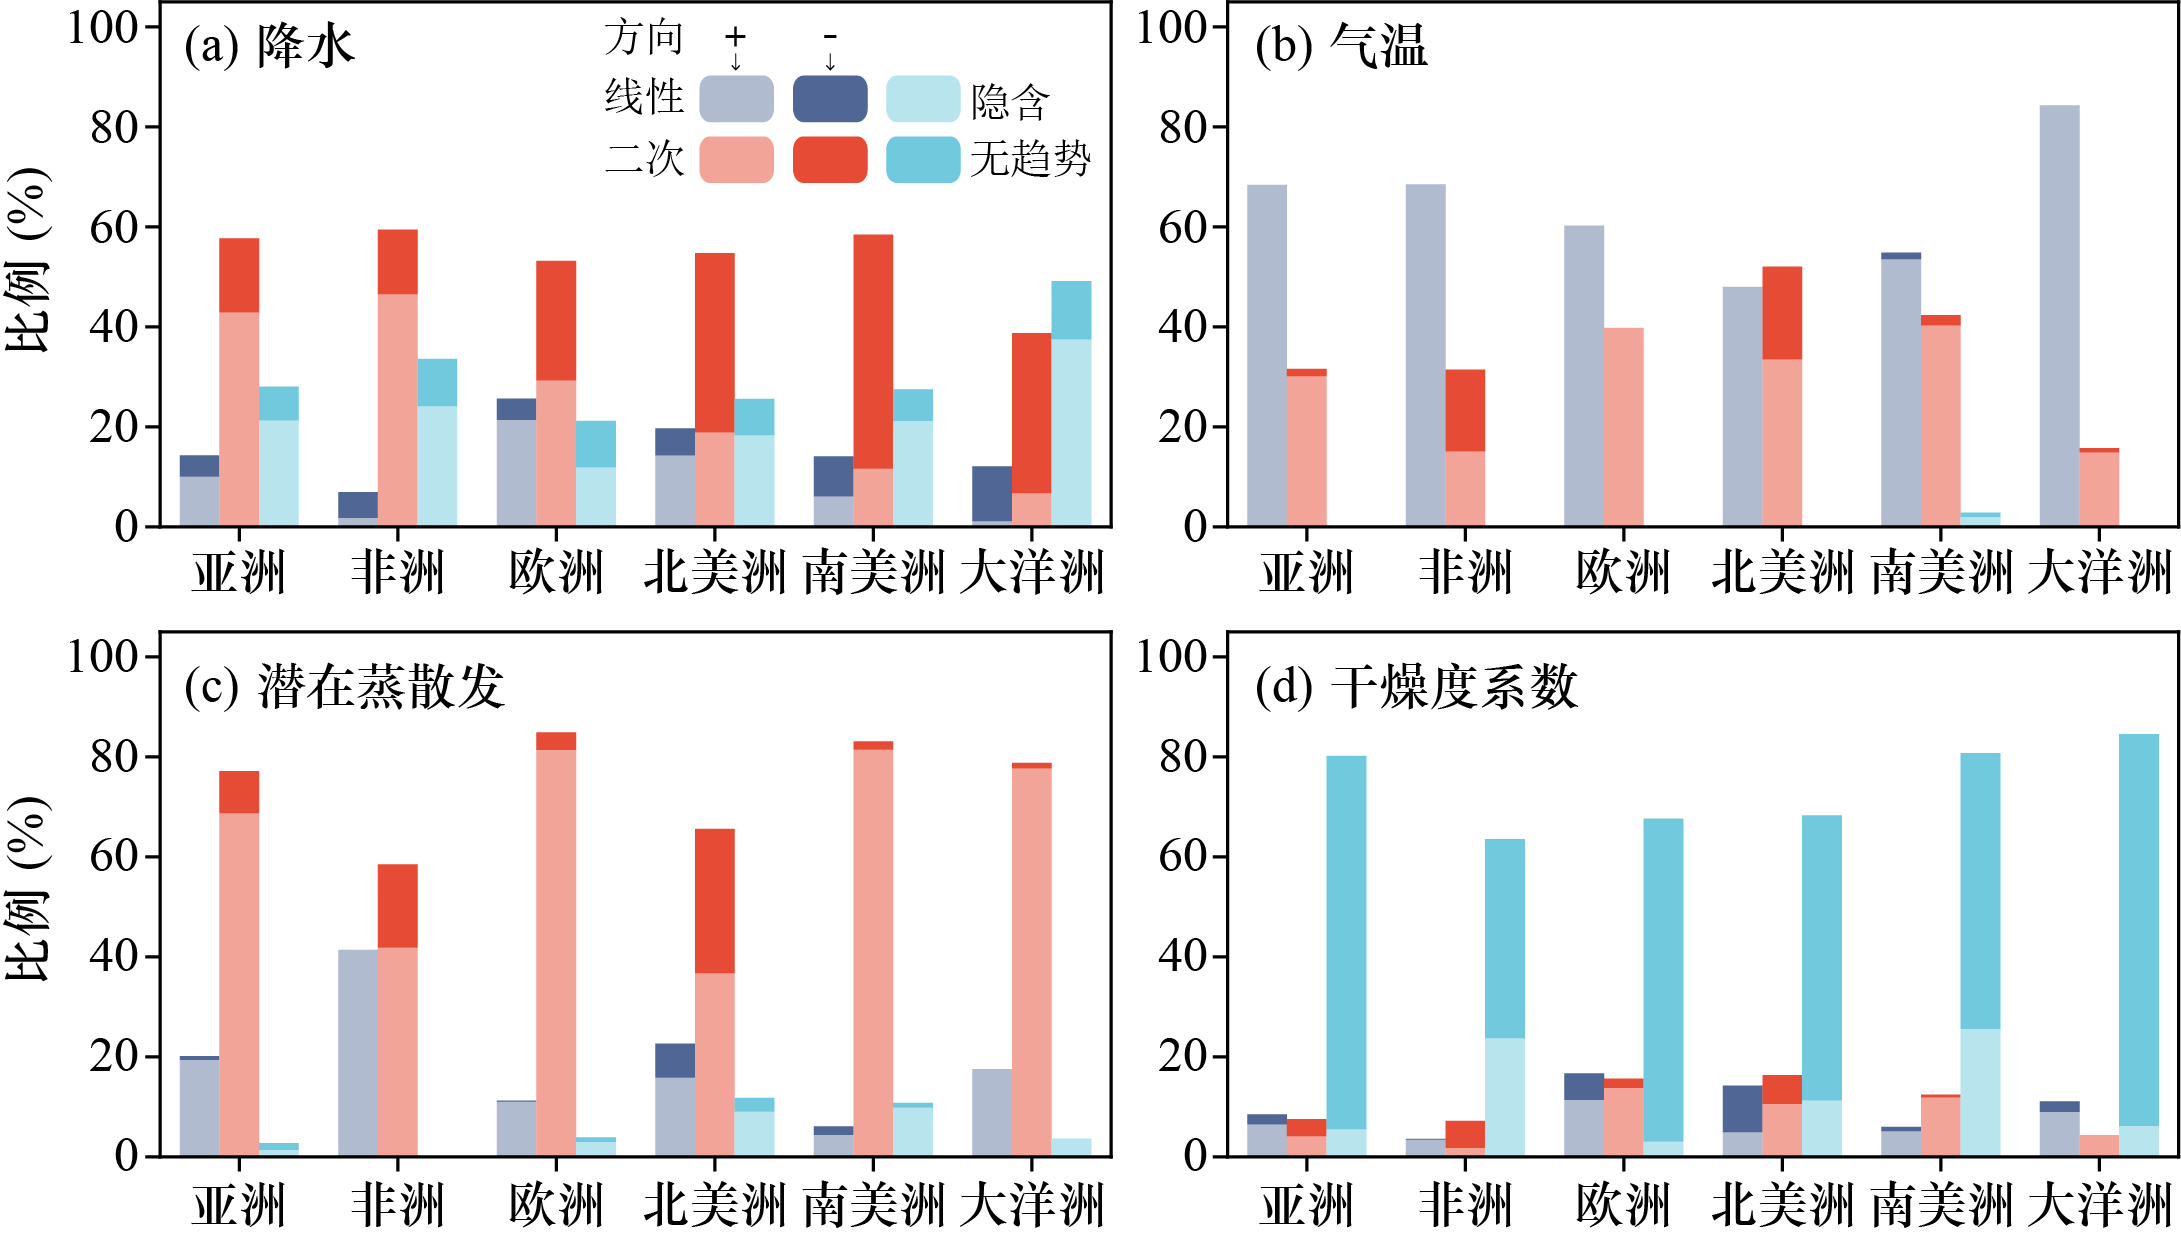
\includegraphics[width=0.85\textwidth]{figures/chap3/1_LNL_Stat_Conti.jpg}
% 	\bicaption{各大洲气候要素线性-非线性变化统计}{Statistic of trend direction and linear-nonlinear trend type for each continents}
% 	\label{fig:LNL_Stat_Conti}
% \end{figure}

% \begin{figure}[H]
% 	\centering
% 	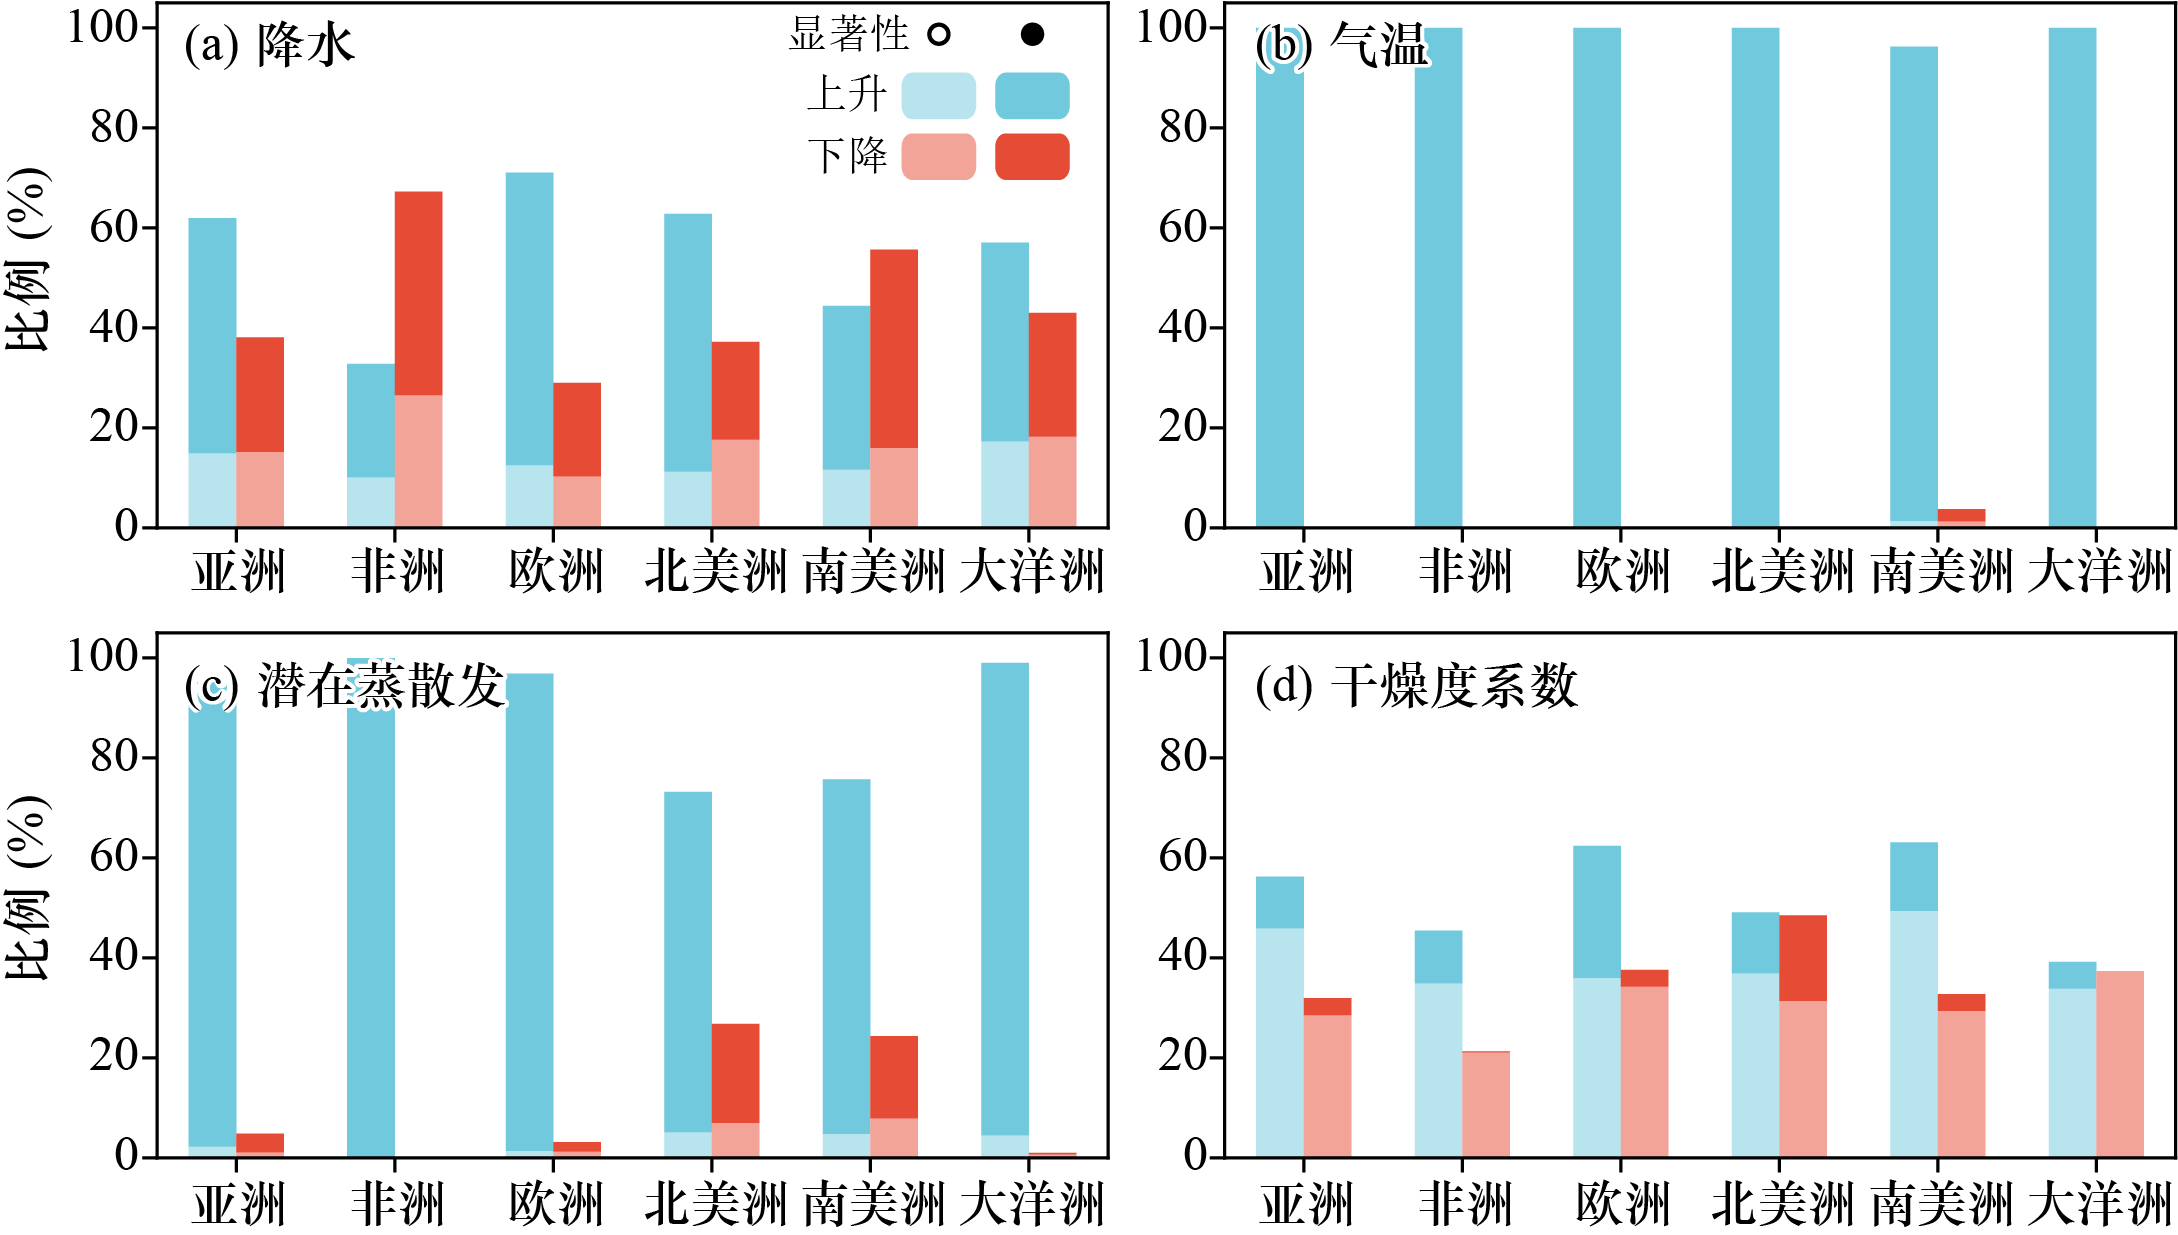
\includegraphics[width=0.85\textwidth]{figures/chap3/1_Trend_Stat_Conti.jpg}
% 	\bicaption{各气候区气候要素线性-非线性变化统计}{Statistic of trend direction and linear-nonlinear trend type for each climatic zones}
% 	\label{fig:LNL_Stat_Clim}
% \end{figure}

% \section{全球历史径流观测演变格局}

% \subsection{研究区域}

% 由于径流序列的分析需要一致的且具有一定长度的时间序列,并且对于缺失值敏感,研究的目的是评估不同区域在不同时间段内的径流演变规律。为了尽可能减少数据缺失和不确定性给分析带来的影响,同时尽量保证测试集水区的选择能够覆盖全球大多数陆地范围,以下5个标准被用于在所有数据集(全球流域数据集中,GRDC提供的10829站点,GSIM提供的30595站点和中国径流数据集中54个站点,共41842各占)中筛选可用于研究的流域。
% \begin{enumerate}
%     \item 删除GSIM与GRDC数据集中的重复站点。在此步骤中,10611个流域被排除在研究区之外。
%     \item 删除数据序列较短的站点,包括:
%     \begin{enumerate}
%         \item 径流序列少于15年。
%         \item 径流序列终止日期早于1900年。
%         \item 径流序列起始日期晚于2000年的站点。
%     \end{enumerate}
%     \qquad 在此步骤中,9983个流域被排除在研究之外。
%     \item 删除数据序列中缺失值较多的站点,包括:
%     \begin{enumerate}
%         \item 数据中NaN(无效值)占比超过50\%。
%         \item 数据中0占比超过50\%。
%         \item 数据中0和NaN总占比超过50\%。
%         \item 连续180个数据中0和NaN占比超过70\%
%         \item 最大值和最小值之差小于2。
%     \end{enumerate}
%     \qquad 在此步骤中,8926个流域被排除在研究之外。
%     \item 删除流域面积小于5km\textsuperscript2的流域以排除过小流域和GSIM中流域边界计算错误。在此步骤中,共有6926个流域被排除在研究之外。
%     \item 删除集水区边界中不包含CRU气候数据格点的站点,以此保证流域气候条件的数据可用性。在此步骤中,955个流域被排除在研究之外。
% \end{enumerate}\par
% 经过上述准测筛选后,共有13627个流域被包含在本章节的研究范围内,如图\ref{fig:Study_Area_Trend}所示。根据Gudmundsson等\cite{gudmundssonObservedTrendsGlobal2019}提出的准则,包含了超过50个研究流域的次大陆区域再研究中被认为是充分的。图中统计了各个区域包含的流域数量,包含了超过50个流域的次大陆区域在图中以红色边框标出,共有31个区域被选出。

% \begin{figure}[H]
% 	\centering
% 	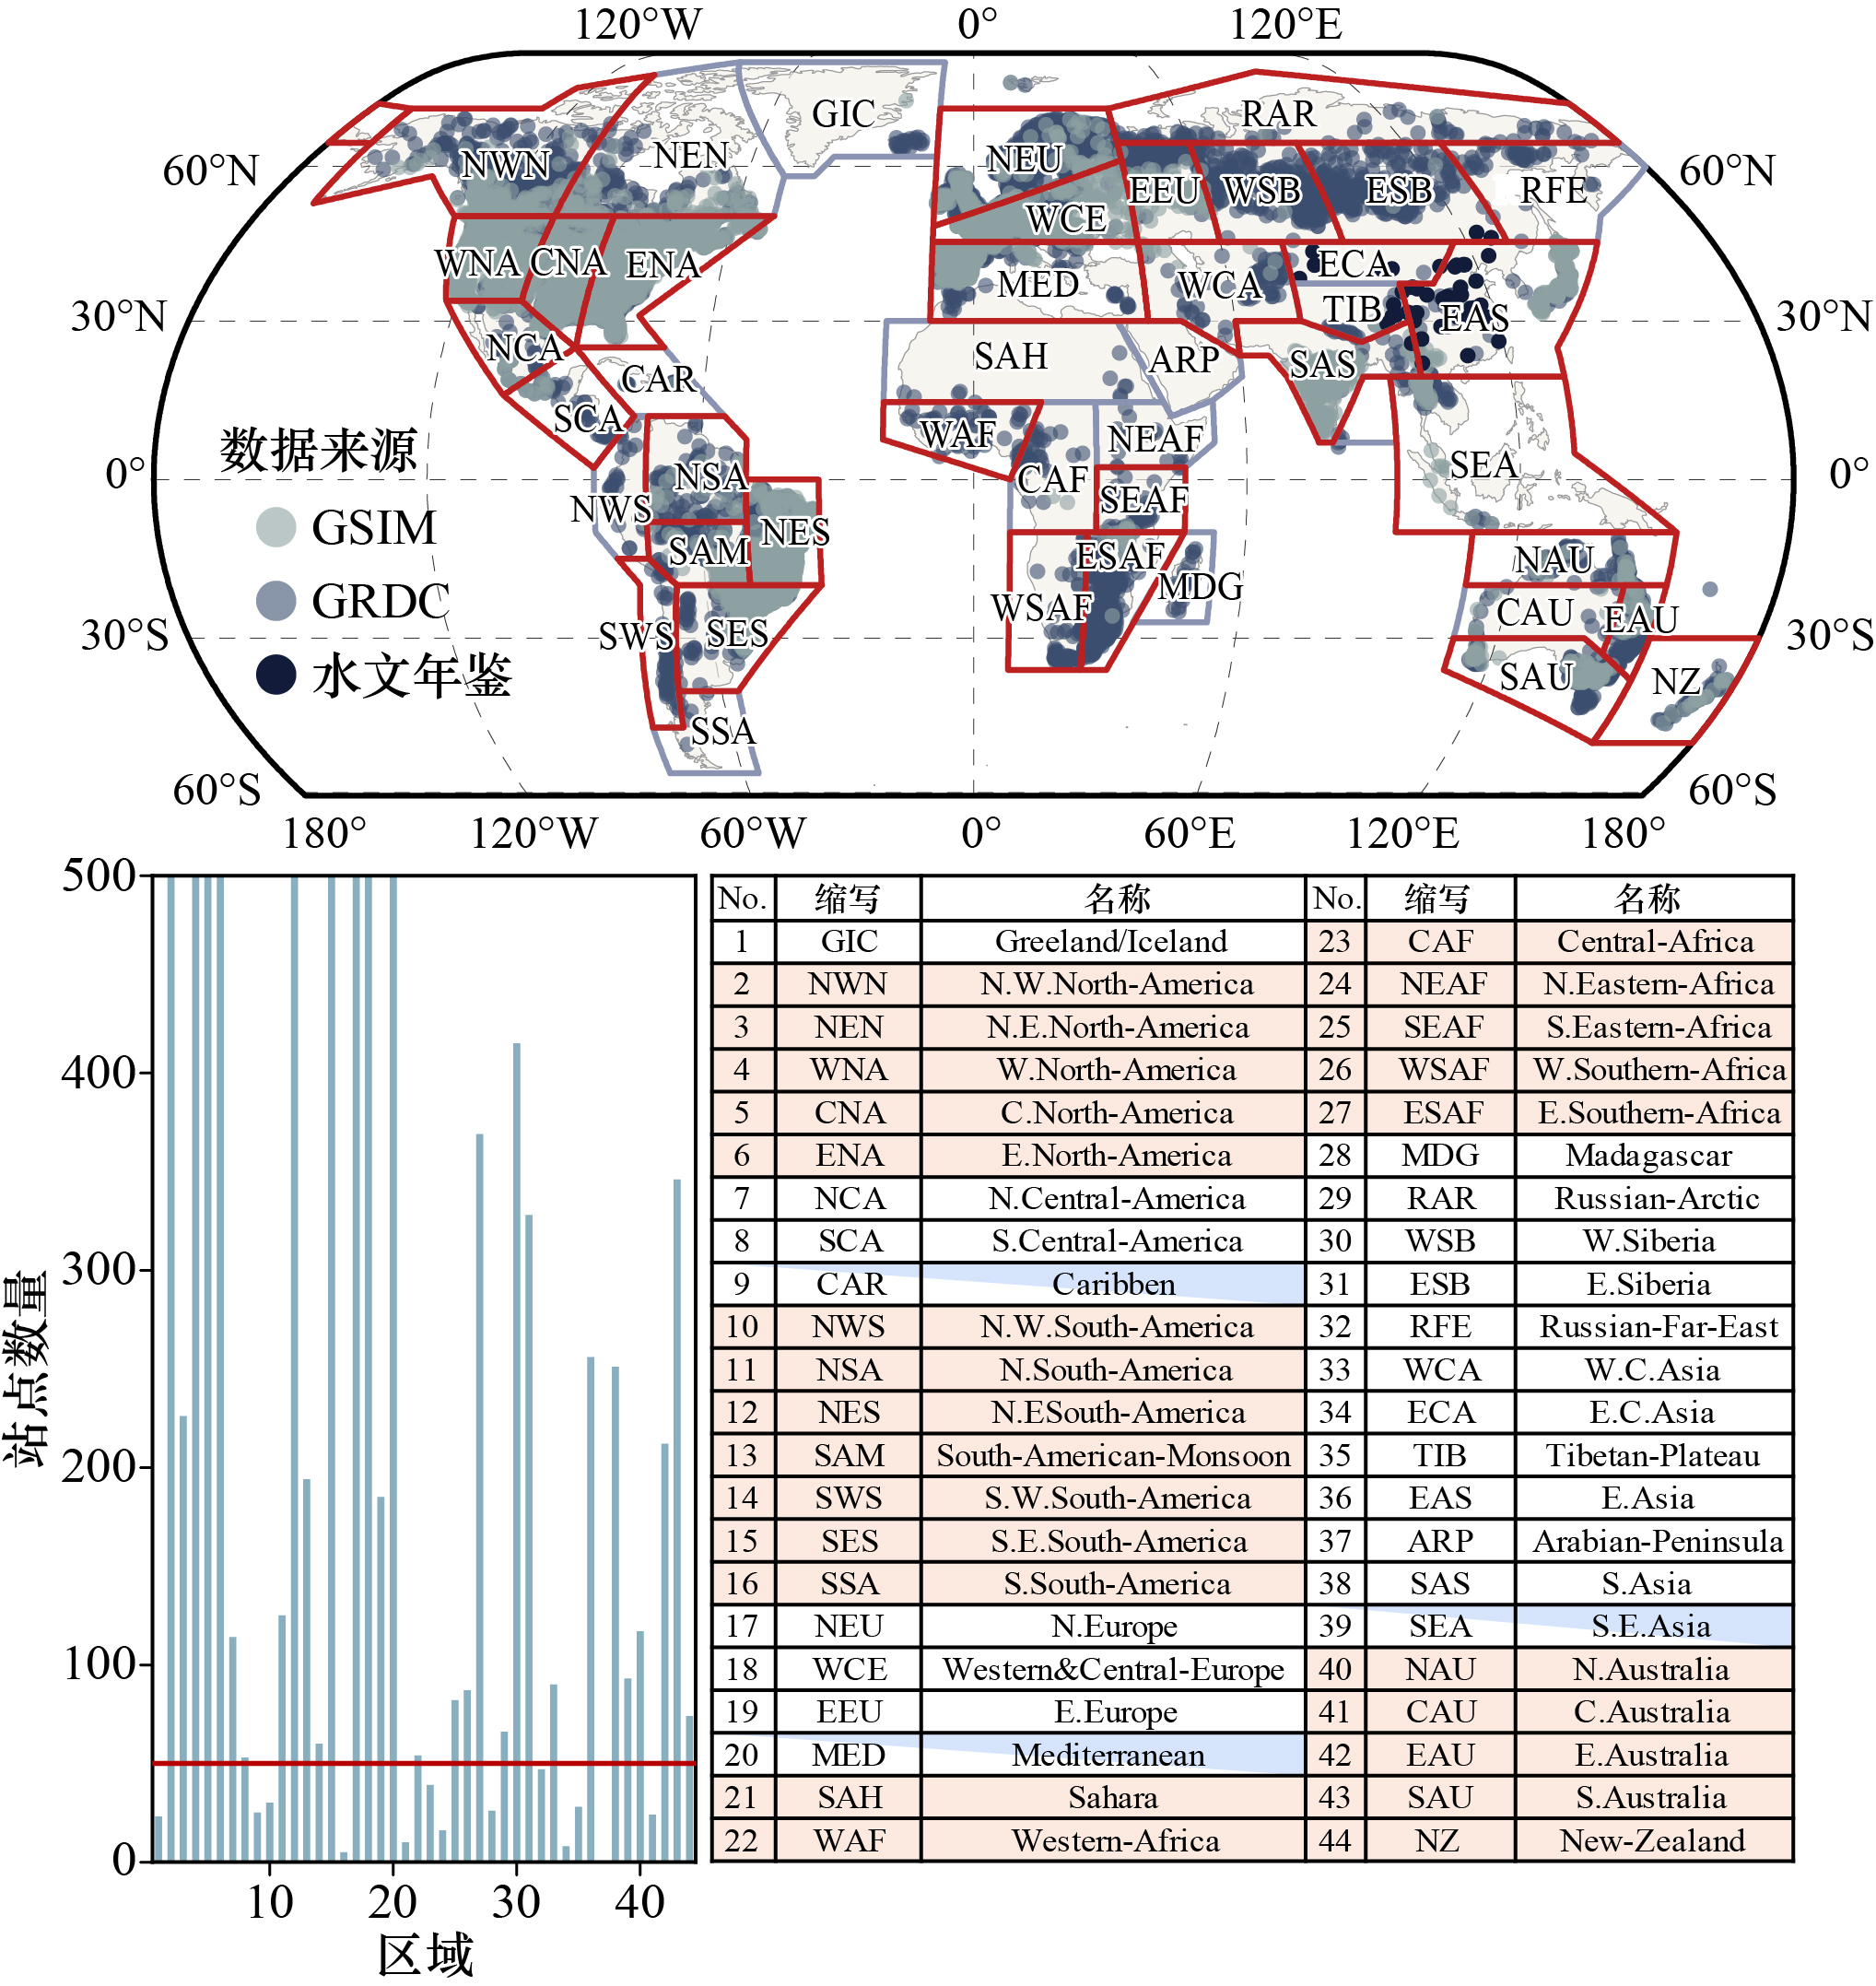
\includegraphics[width=0.85\textwidth]{figures/chap3/0_Study_Area_Trend.jpg}
% 	\bicaption{研究流域分布图}{Map of catchments involved in this chapter}\label{fig:Study_Area_Trend}
% \end{figure}

% \subsection{实测径流数据缺失值插补}

% 本节对全球范围内10799个流域的径流数据进行了缺失值和无效值的插补,平均缺失率为7.1\%,目的是保证BFAST算法的准确执行。对于每个流域,分别训练了三种机器学习模型,模型在训练集和测试集上的评估指标如图\ref{fig:Interp_Indices_Boxplot}所示。从NSE来看,三种模型在训练集上的表现都比较好,均在超过一半的流域得分超过0.5,其中XGB的表现最为优越,在超过75\%的流域中NSE超过了0.7。测试集上的表现相对于测试集较差,NSE普遍低于训练集,表明模型在测试集上的泛化能力有所降低,其中,XGB的性能下降最为明显,其次是RF,SVR的性能下降不显著,说明XGB的过拟合现象较为明显。从RE来看,RF和XGB在训练集都能比较精确的模拟出径流的水量特征,而SVR则存在明显的低估,在超过一半的流域径流模拟偏差超过了10\%。RMSE和CC指标表现出的规律与NSE和RE类似。三种模型在测试集上的表现比较相似,XGB在训练集上的性能最好,RF具有最高的稳定性,几乎不存在过拟合现象。\par

% \begin{figure}[H]
% 	\centering
% 	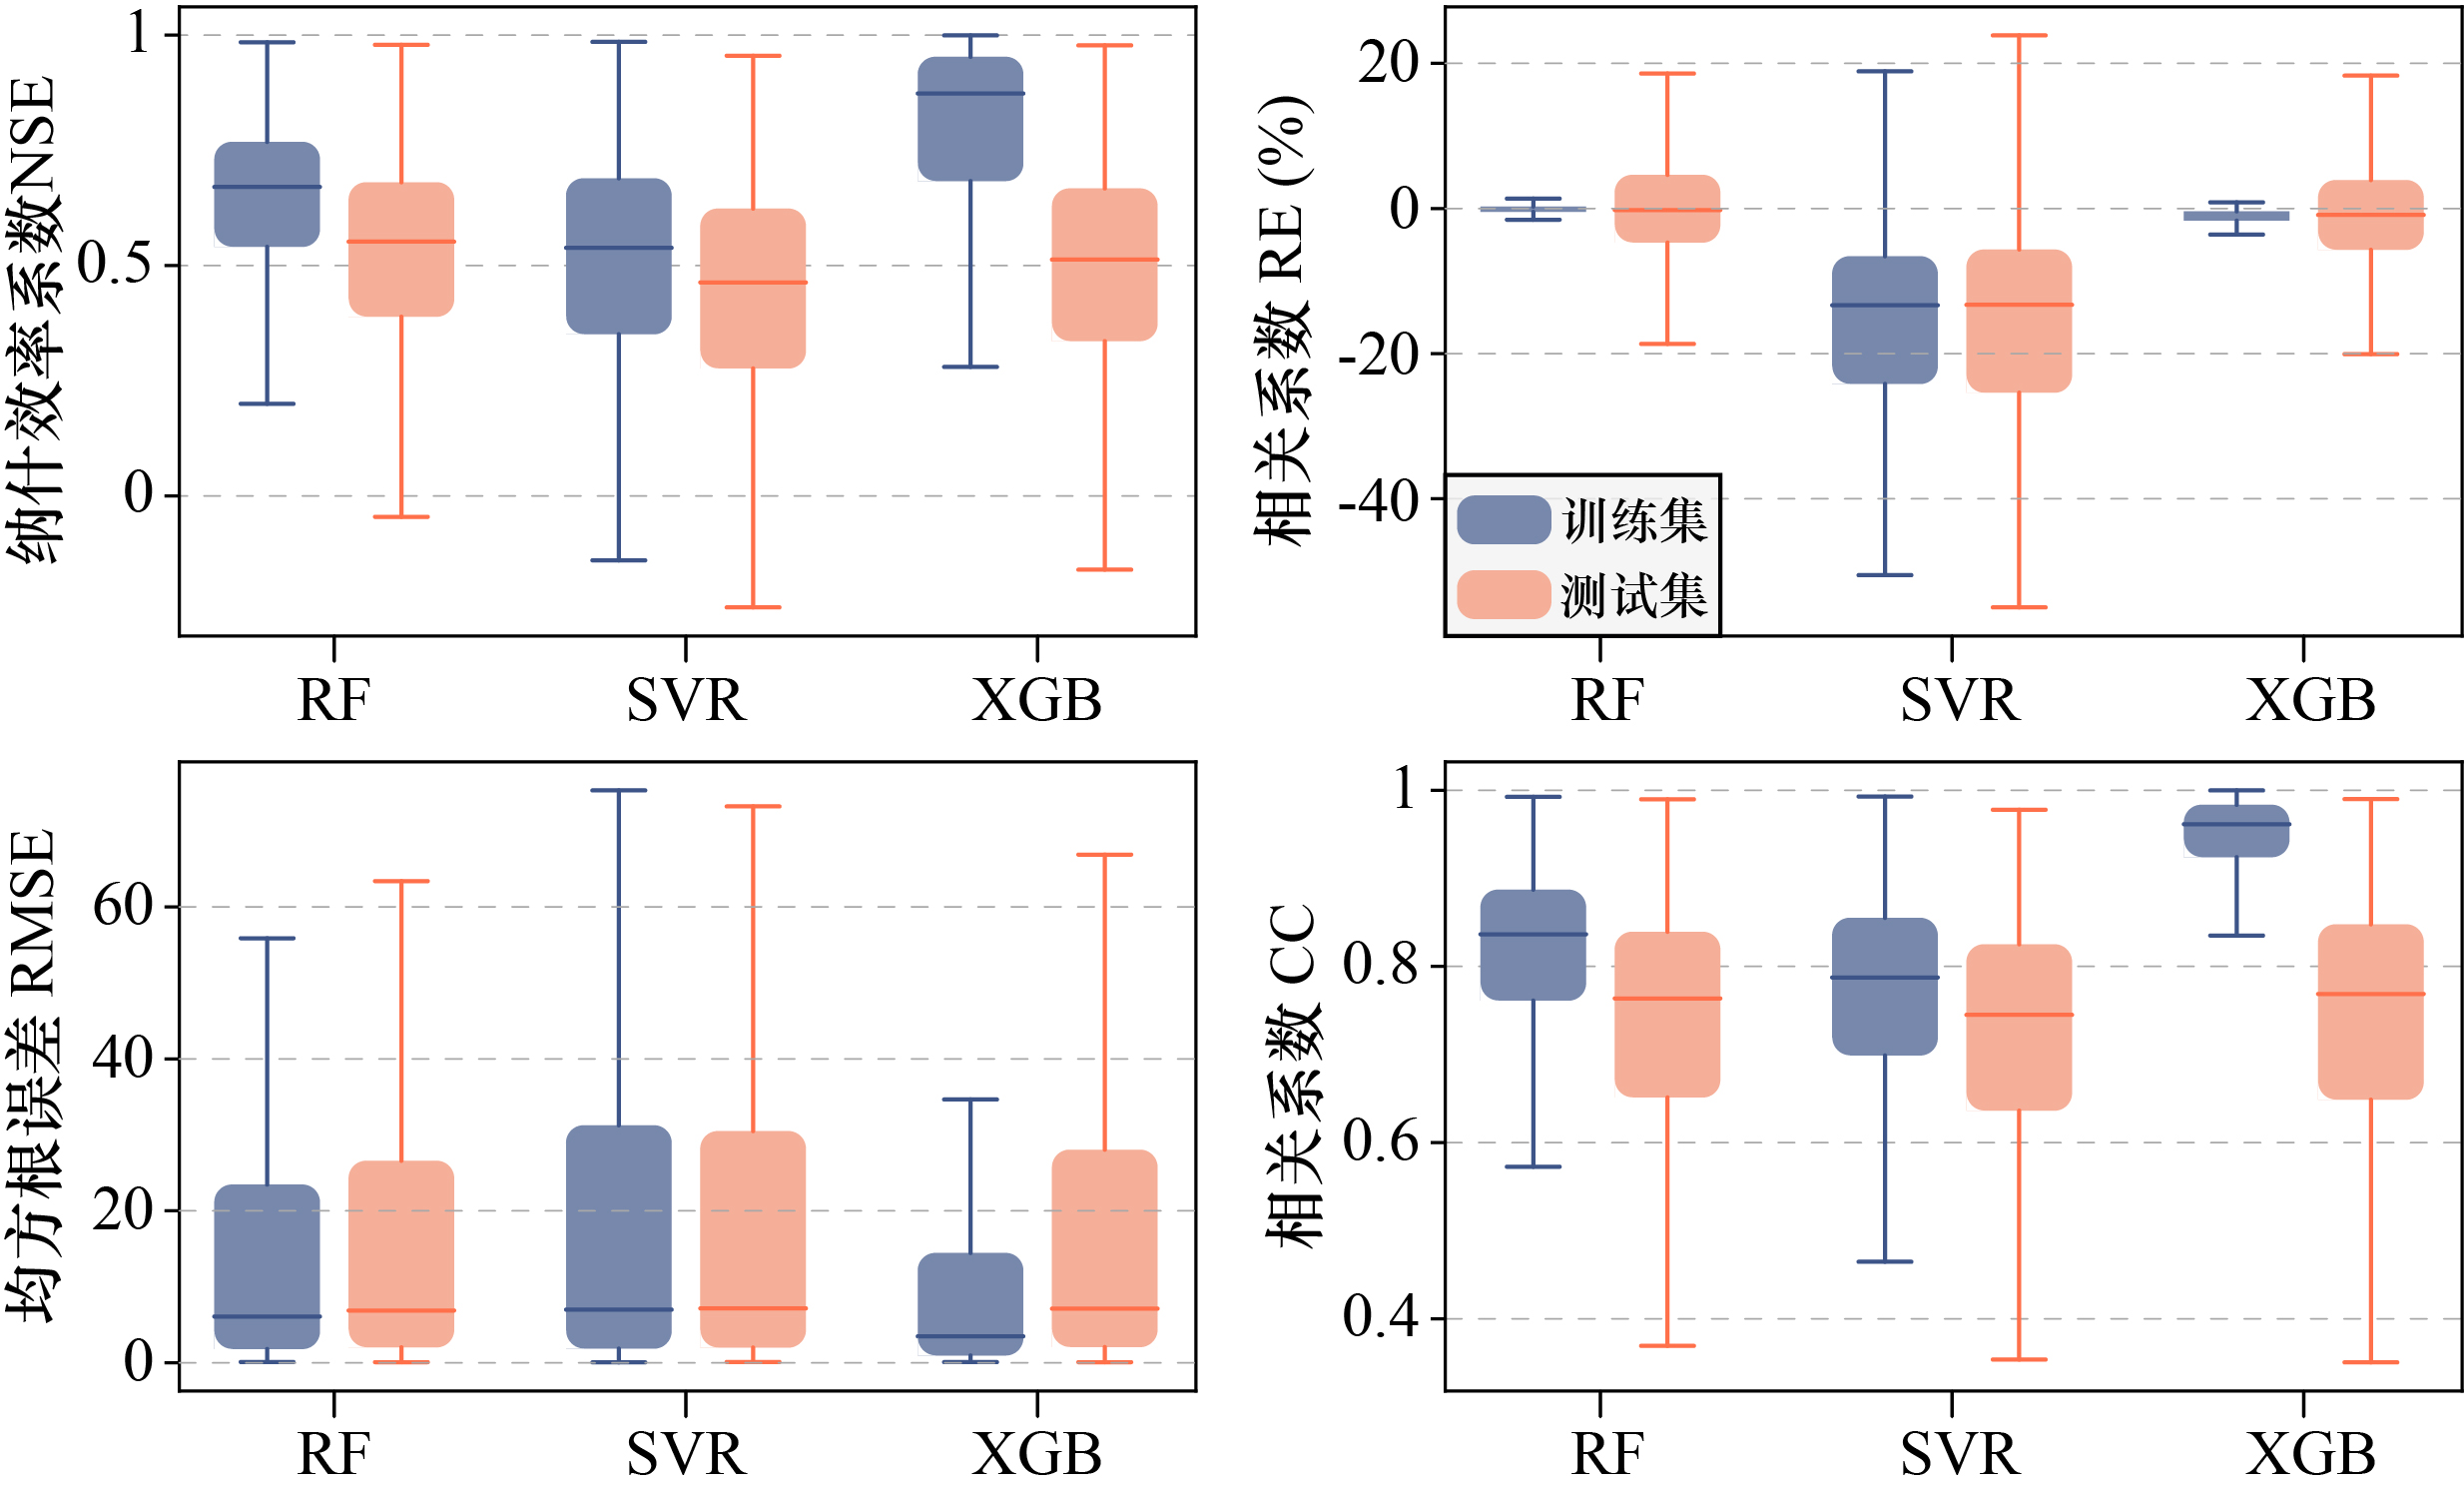
\includegraphics[width=0.85\textwidth]{figures/chap3/2_Interp_Indices_Boxplot.jpg}
% 	\bicaption{三种机器学习模型在训练集和测试集下的四种评估指标统计结果}{Four performance indices for three ML models in train set and test set}
%   \label{fig:Interp_Indices_Boxplot}
% \end{figure}

% 如图\ref{fig:Interp_TrTe_NSE_RE}所示,空间上看,RF和XGB在各个区域流域的测试集上表现都很好,大多数流域的NSE值都在0.6以上,尤其是在欧洲、北美和中国部分地区,但是在测试集的表现上,模型性能存在明显的空间异质性。在北美洲中部、欧洲东南部、大洋洲东南部等较为干旱的区域,模型的模拟结果较为失败,可能是由于这些地区复杂的水循环过程难以用简单的非线性机器学习模型进行概括\cite{ghiggiGRUNObservationbasedGlobal2019}三种模型在训练集上的RE值较低,大多数流域的RE值集中在-5\%到5\%之间,偏差较小。对于SVR来说,训练集和测试集的表现差异不大,但总体呈现低估径流的现象,特别是在高流量部分,在北美洲东部和西部、欧洲西部、南美洲东部、非洲中南部、亚洲东部和北部等区域的模拟较为成功。散点图进一步验证了前面的结论。XGBoost在训练集和测试集上的拟合线都非常接近对角线,表明其预测值与观测值之间的偏差最小。随机森林的散点图在测试集上稍微偏离对角线,但总体表现还算稳定。SVR的散点图偏离对角线最为明显,尤其在测试集上,显示出较大的预测误差。\par

% \begin{figure}[H]
% 	\centering
% 	\includegraphics[width=0.9\textwidth]{figures/chap3/2_Interp_TrTe_NSE_RE.jpg}
% 	\bicaption{三种机器学习模型在训练集和测试集下的NSE和RE指标空间分布}{Spatial patterns of NSE and RE score for three ML models in train set and test set}
%   \label{fig:Interp_TrTe_NSE_RE}
% \end{figure}

% 将基于机器学习模型预测的径流缺失值插入原径流序列的对应位置,并且对比两个序列的径流量的相对误差和标准差的相对误差,如图\ref{fig:Interp_RE_Bef_Aft}所示。从图中可以看出,插补后的径流量序列与原始序列的相对误差普遍较小,大部分流域的相对误差小于5\%,标准差的相对误差也普遍较小,但是主要呈现负偏差,说明相比于原径流序列,插补后的径流序列的变异性较小。总体来看,插补后的径流序列与原始序列的特征较为接近,原始序列的径流特征得以保留,可以用于后续的研究。\par

% \begin{figure}[H]
% 	\centering
% 	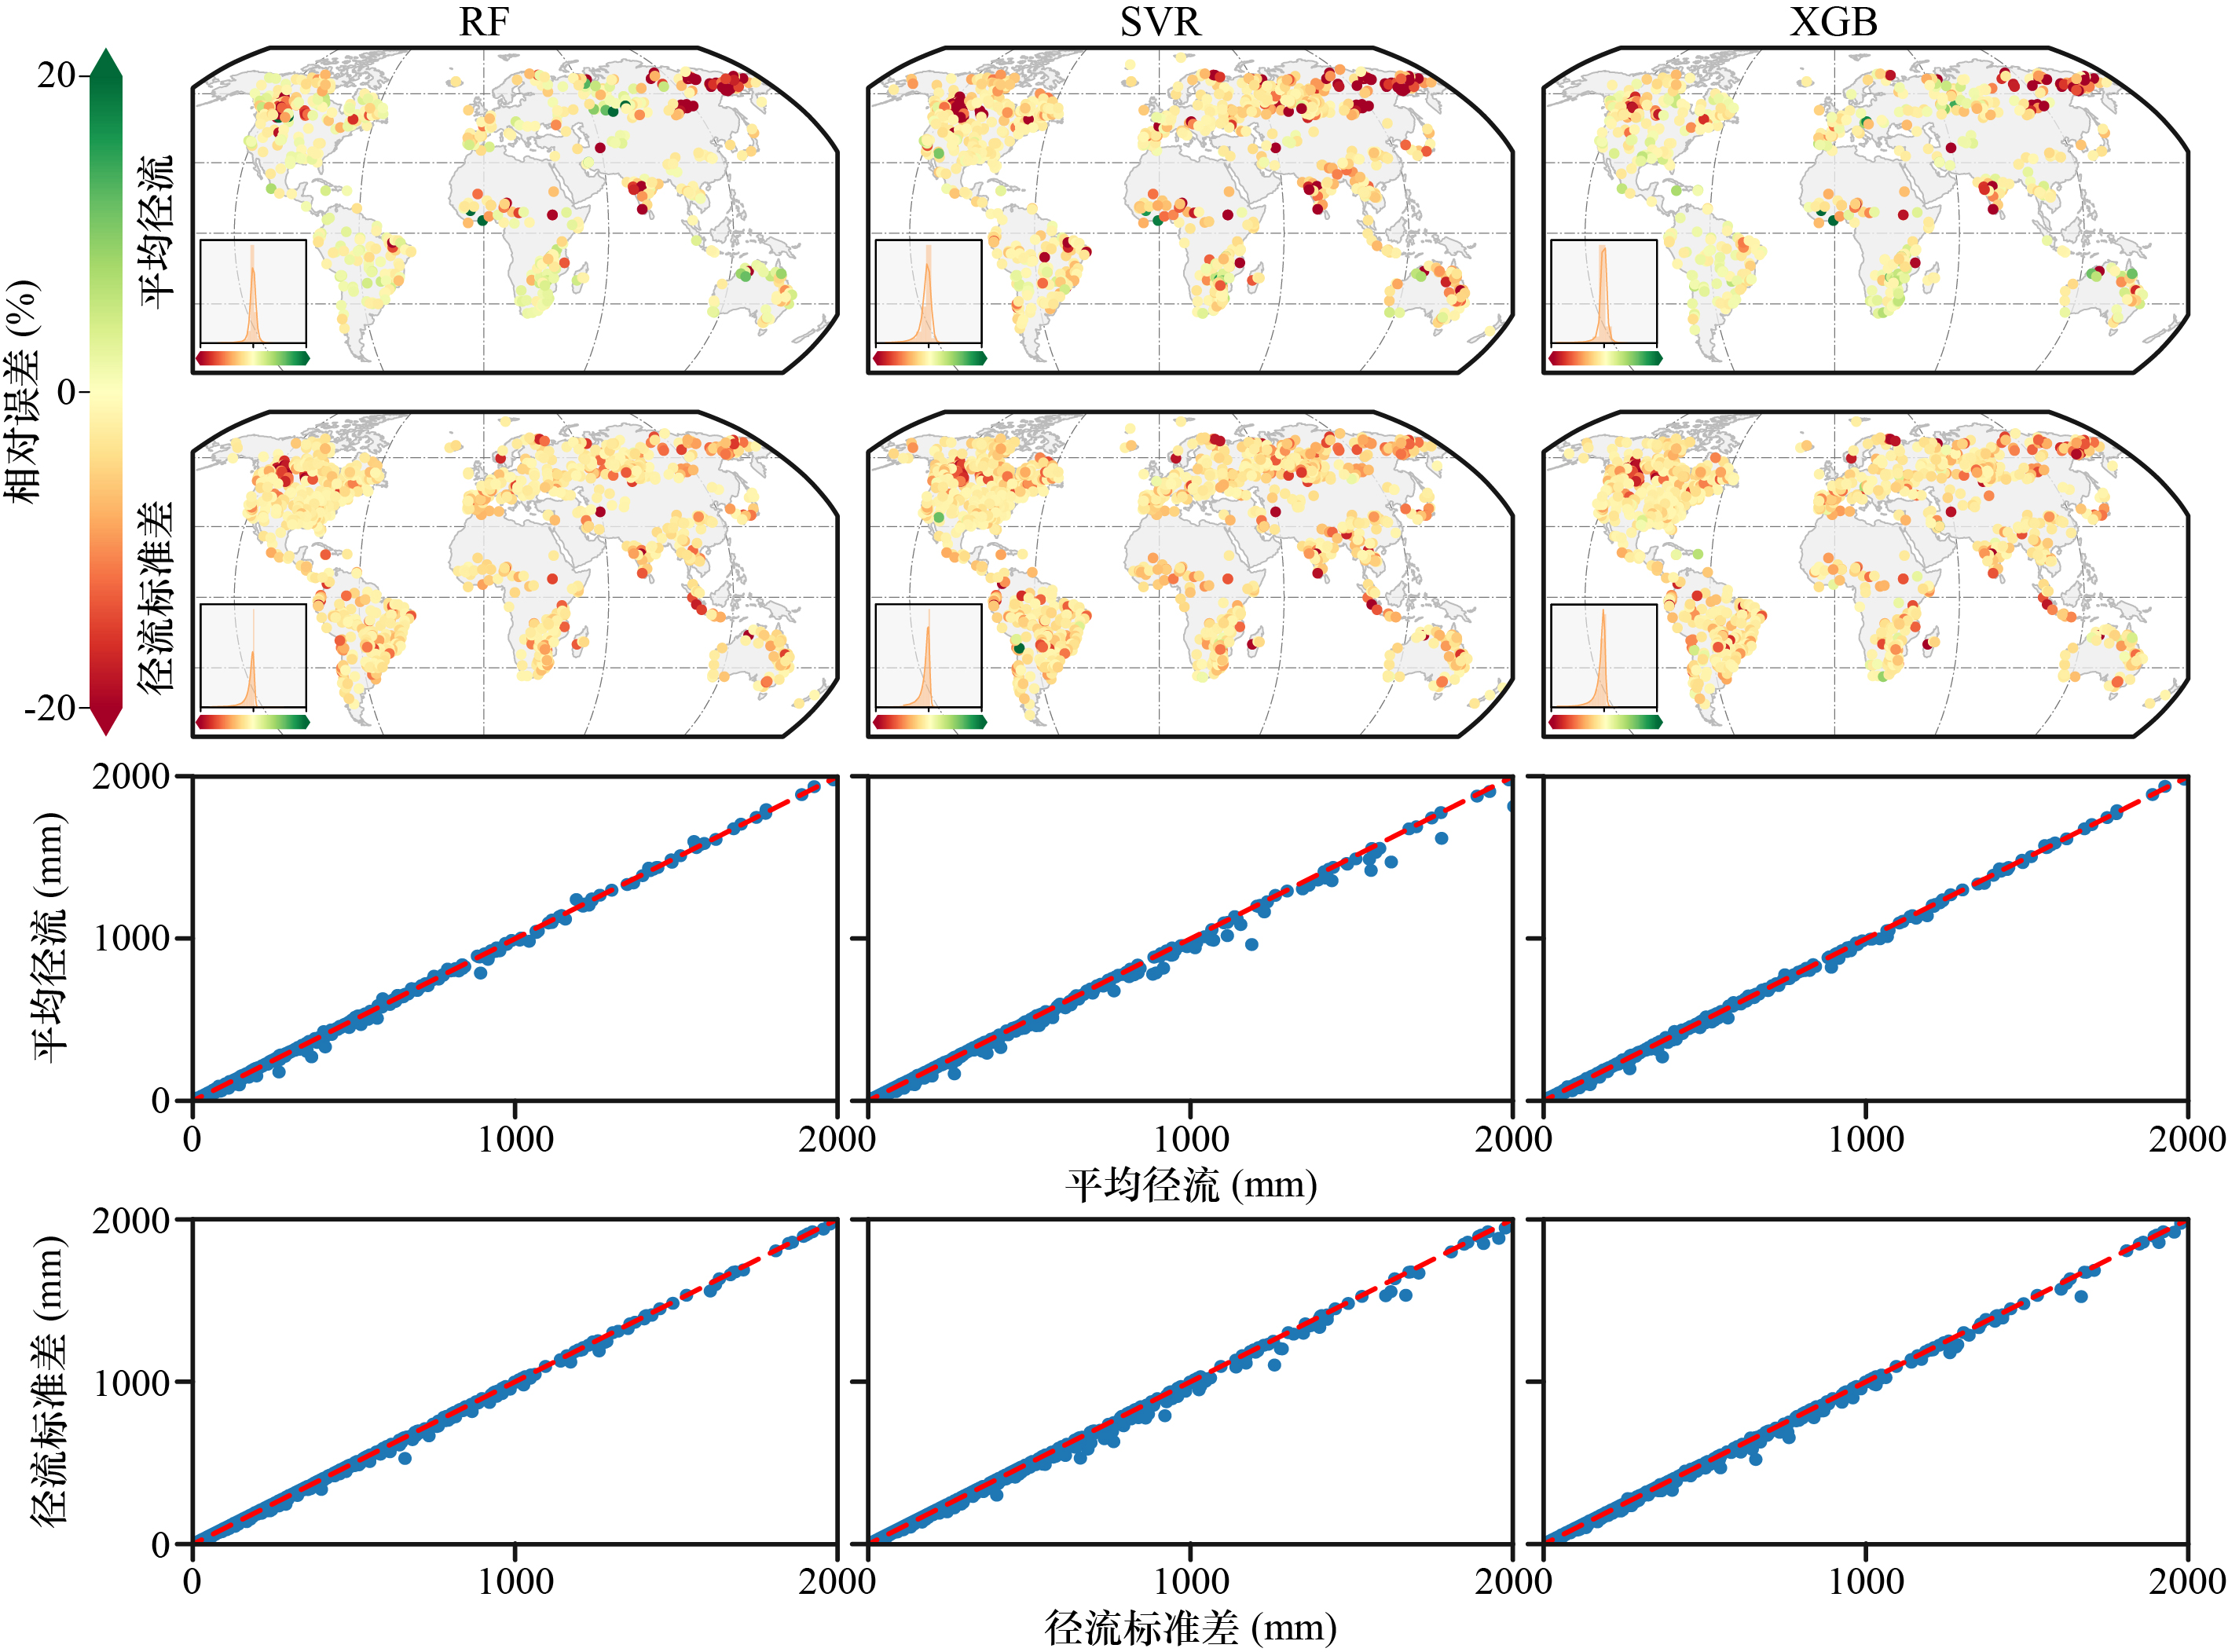
\includegraphics[width=0.9\textwidth]{figures/chap3/2_Interp_RE_Bef_Aft.jpg}
% 	\bicaption{数据插补前后径流量的相对误差和标准差的相对误差}{Relative error of runoff standard deviation between before and after the interpolation}
%   \label{fig:Interp_RE_Bef_Aft}
% \end{figure}

% \subsection{径流历史序列断点特征}

% \begin{figure}[H]
% 	\centering
% 	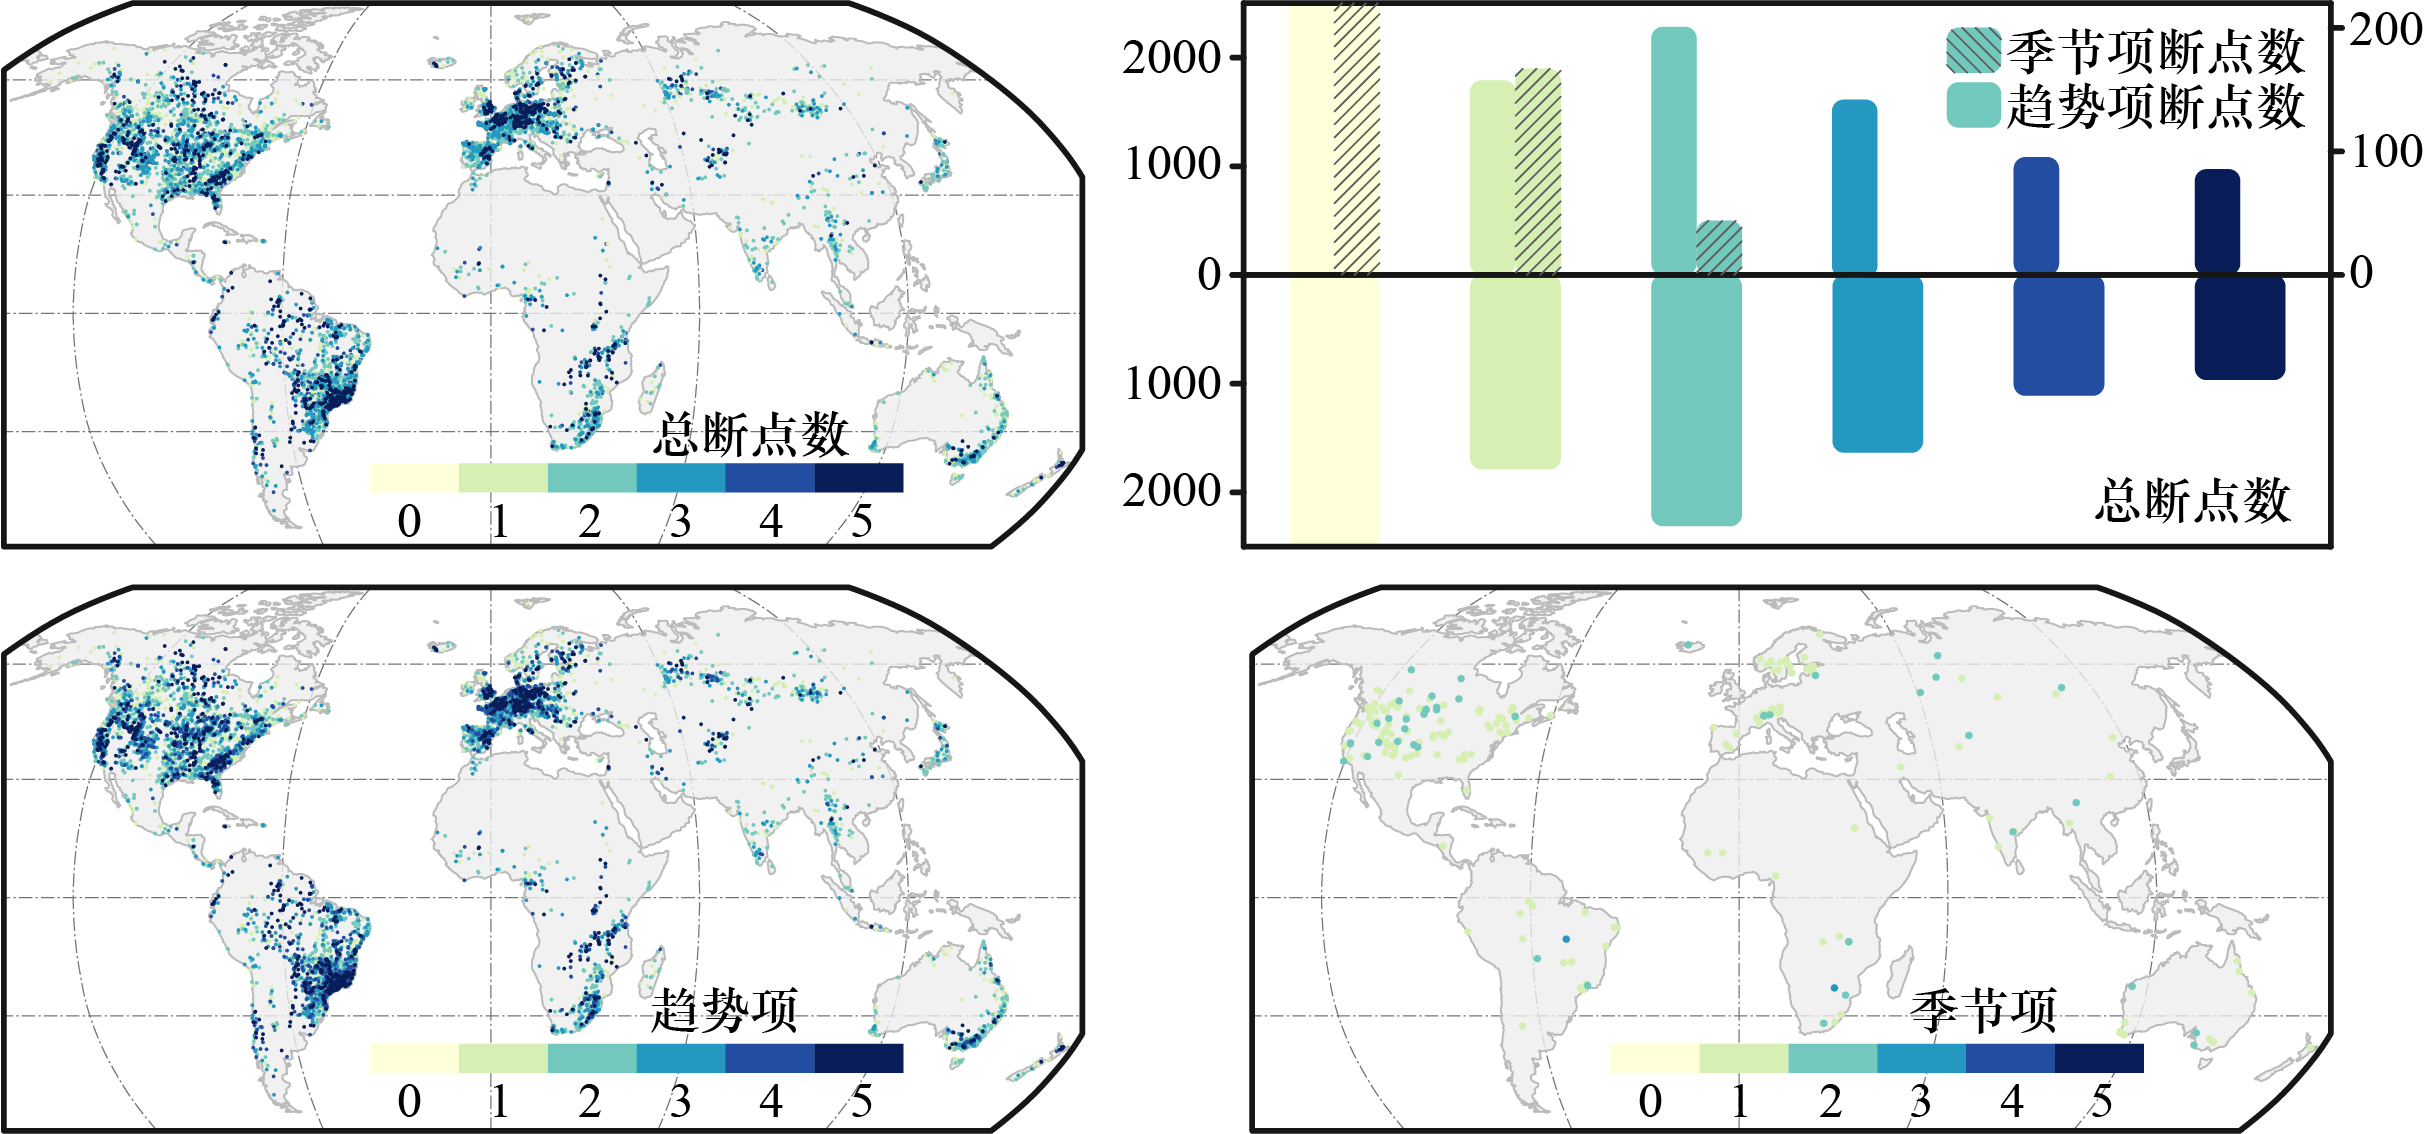
\includegraphics[width=0.8\textwidth]{figures/chap3/3_RUN_BP_Num.jpg}
% 	\bicaption{全球历史径流序列断点数量}{Breakpoints number in global historical runoff series}
%   \label{fig:RUN_BP_Num}
% \end{figure}

% \begin{figure}[H]
% 	\centering
% 	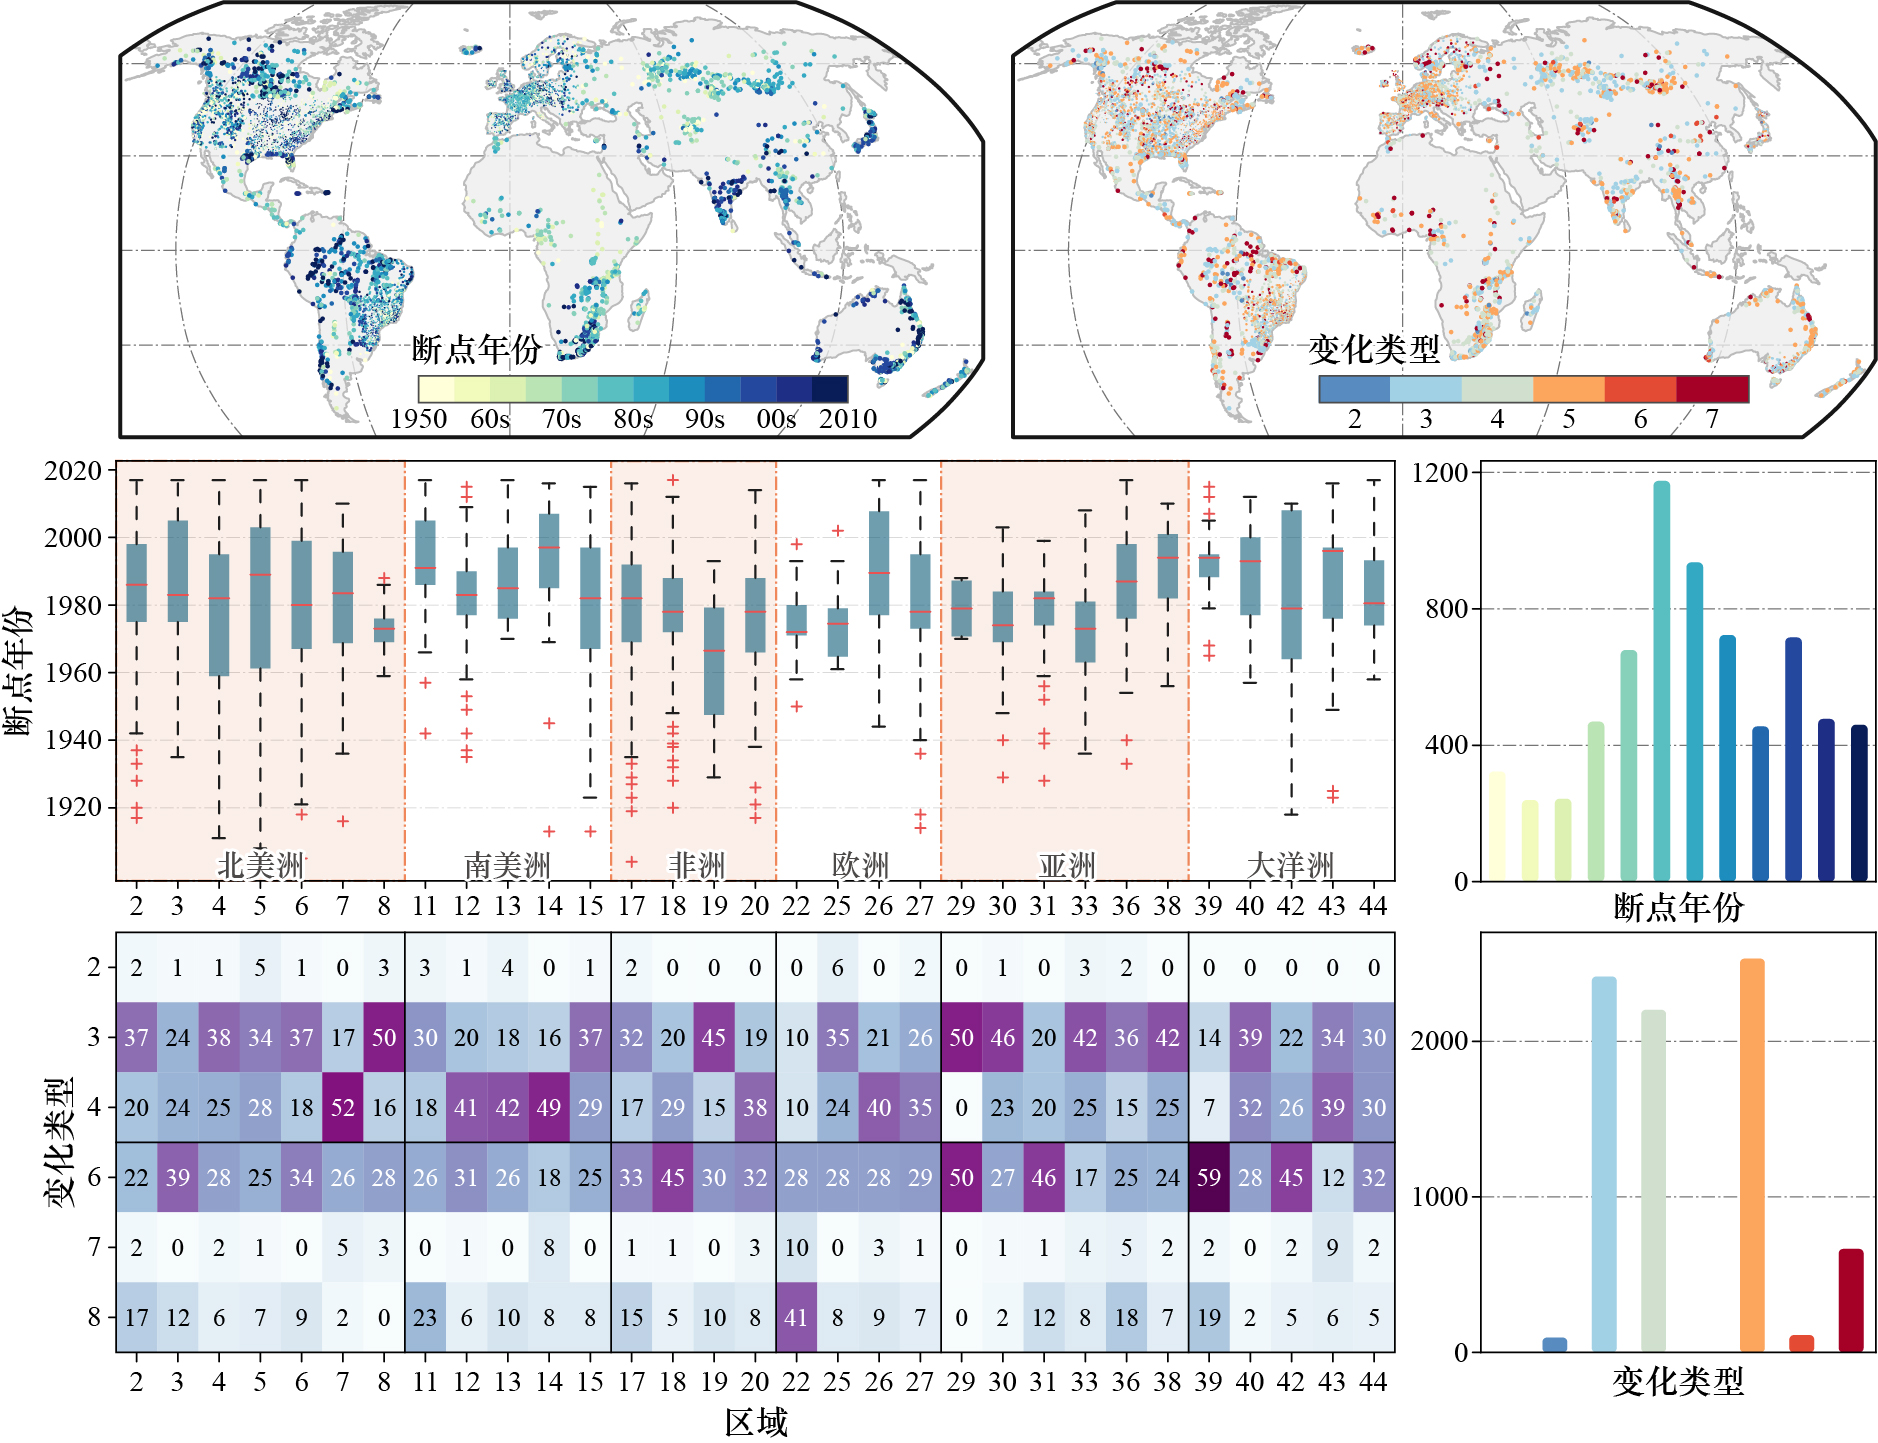
\includegraphics[width=0.9\textwidth]{figures/chap3/3_RUN_BT_Class.jpg}
% 	\bicaption{径流序列断点时间及序列变化特征}{Breakpoints time and change type before and after the breakpoint}
%   \label{fig:RUN_BT_Class}
% \end{figure}

% \subsection{全球陆地径流演变趋势}

% \section{多时空尺度径流变化归因分析}

% \section{讨论}

% \section{本章小结}
